%%%%%%%%%%%%%%%%%%%%%%%%%%%%%%%%%%%% Chapter Template

\chapter{2D steady simulations} 	% Main chapter title
\label{Chapter1} 		% For referencing the chapter elsewhere, usage \ref{Chapter1}

%%%%%%%%%%%%%%%%%%%%%%%%%%%%%%%%%%%%

The initial goal was to identify the factors that contribute to the VMG's superior efficiency compared to the R1V4 and make the necessary adjustments.

The first step involved identifying the parameters that respond to various flight conditions. Following that, a low-fidelity approach using XFLR5 was employed to compute the 2D aerodynamic coefficients, providing insights into the disparities between the airfoils. Subsequently, Fluent CFD software was utilized to obtain a more precise assessment of the aerodynamic coefficients for each airfoil during actual flight conditions.

%%%%%%%%%%%%%%%%%%%%%%%%%%%%%%%%%%%%%%%%%%%%%%%%%%%%%%%%%%%%%%%%%%%%%%%%%%%%%%%%
%%%%%%%%%%%%%%%%%%%%%%%%%%%%%%%%%%%% SECTION 1 %%%%%%%%%%%%%%%%%%%%%%%%%%%%%%%%%
%%%%%%%%%%%%%%%%%%%%%%%%%%%%%%%%%%%%%%%%%%%%%%%%%%%%%%%%%%%%%%%%%%%%%%%%%%%%%%%%

\section{Kite flight modelling}
\label{sec:Ch1.1}

The kite is modelized according to the "zero mass model" as developed in the course given by Richard Leloup in Supaero \cite{cours_leloup}.

\begin{figure}[H]
    \centering
    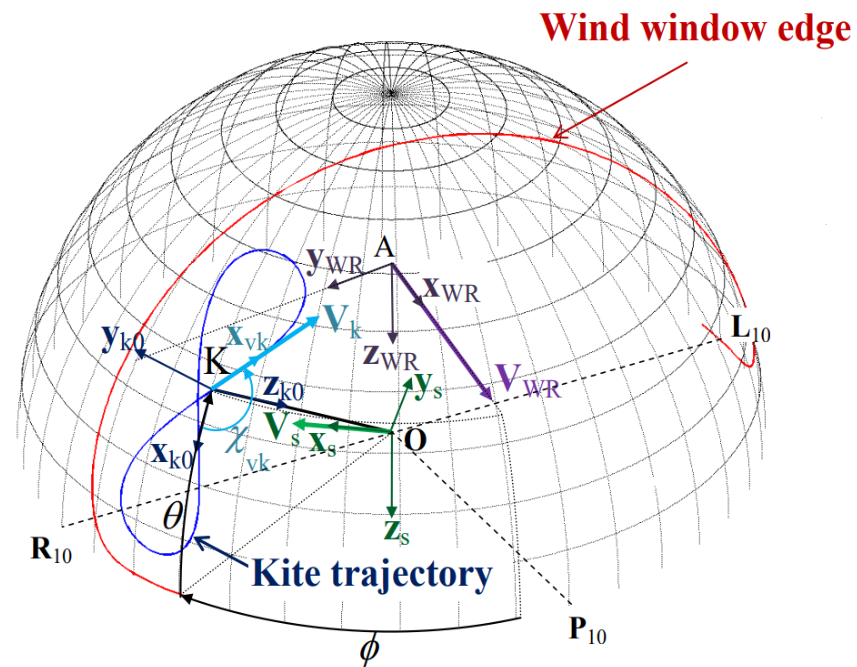
\includegraphics[width=0.7\textwidth]{figures/2D steady simulations/kite flight modeling 1.png}
    \caption{Speeds \& angles decomposition}
    \label{fig:Kite_flight_modelling}
\end{figure}

\begin{figure}[H]
    \centering
    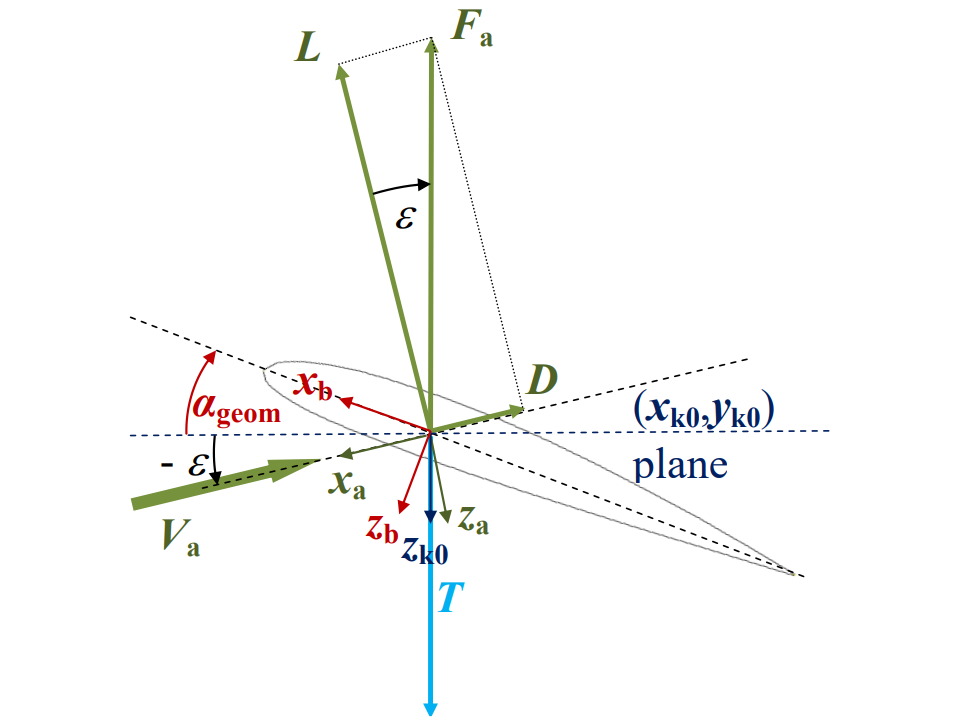
\includegraphics[width=0.8\textwidth]{figures/2D steady simulations/kite flight modeling 2.png}
    \caption{Decomposition of the aerodynamic force vector}
    \label{fig:Kite_flight_modelling}
\end{figure}

The Zero-mass model approach leads to the following results : 
\begin{equation}
\left \{
   \begin{array}{r c l}
      V_{WR}  & = & V_{WT} - V_{S} \\
      V_{a}   & = & V_{WR} - V_{k} \\
      F_{a} & = & -T = \frac{1}{2}\frac{C_{L} \rho A V_{a}^{2}}{cos(\epsilon)}
   \end{array}
   \right .
   \label{kite_speed_vectors}
\end{equation}

with, in our case of study, $V_{k} = 0$. As a matter of fact, we are assuming that the kite is static in relation to the ship (the rider). 


Then, we can deduce from the relation \ref{kite_speed_vectors} : 
\begin{equation}
\left \{
   \begin{array}{r c l}
      V_{a}  & = & \sqrt{V_{WT}^2 + V_{S}^2 - 2V_{WT}V_{S}cos(\alpha_{S, WT}) } \\
      \epsilon   & = & \alpha_{S, WT} - \alpha_{a, WT} \\
      \alpha_{a, WT} & = & arctan(\frac{V_{s}sin(\alpha_{S, WT})}{V_{s}cos(\alpha_{S, WT}) - V_{WT}})
   \end{array}
   \right .
   \label{kite_speed_vectors_2}
\end{equation}


\begin{wrapfigure}{r}{0.6\textwidth}
\centering
    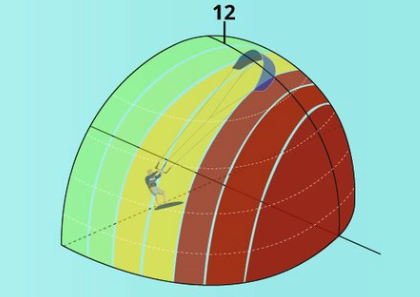
\includegraphics[width=0.5\textwidth]{figures/2D steady simulations/kite flight modeling 3.png}
    \caption{The wind window}
    \label{fig:The_wind_window}
\end{wrapfigure}

Then, we understand that depending on the position of the kite ($\Phi, \Theta$), the rider's speed ($V_{s}$) and the true wind speed ($V_{WT}$), the tether tension (T) is very different. This result has lead to the definition of the wind window represented on the figure \ref{fig:The_wind_window}.

The concept of the wind window holds significant importance in kitesurfing as it presents riders with a fundamental trade-off: the closer the kite is positioned to the center of the wind window, the more power it generates. However, this ideal kite placement might not align with the rider's intended direction. As a result, kitesurfers must strategically position their kites within the wind window to maximize power in their desired direction.


%%%%%%%%%%%%%%%%%%%%%%%%%%%%%%%%%%%%%%%%%%%%%%%%%%%%%%%%%%%%%%%%%%%%%%%%%%%%%%%%
%%%%%%%%%%%%%%%%%%%%%%%%%%%%%%%%%%%% SECTION 2 %%%%%%%%%%%%%%%%%%%%%%%%%%%%%%%%%
%%%%%%%%%%%%%%%%%%%%%%%%%%%%%%%%%%%%%%%%%%%%%%%%%%%%%%%%%%%%%%%%%%%%%%%%%%%%%%%%
\section{The different phases}
\label{sec:Ch1.3}

A kite race is segmented into distinct phases, each corresponding to varying inlet conditions. What's of primary importance for the riders during these phases is their "Velocity Made Good," often referred to as VMG, which signifies their speed aligned with the axis they intend to follow (the wind axis).

\begin{figure}[H]
    \centering
    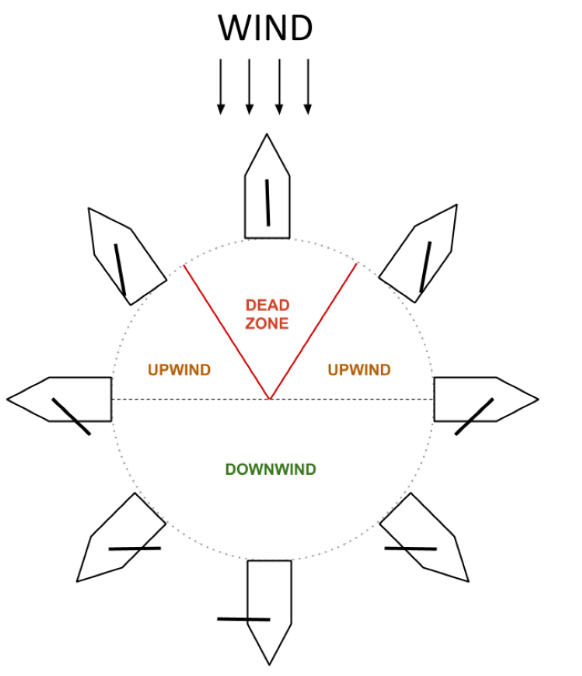
\includegraphics[width=0.5\textwidth]{figures/2D steady simulations/upwind_downwind_scheme.png}
    \caption{Upwind and downwind diagram}
    \label{fig:upwind_downwind_scheme}
\end{figure}

%%%%%%%%%%%%%%%%%%%%%%%%%%%%%%%%%%%% SUBSECTION 1

\subsection{The upwind}
\label{sub:Ch1.3.1}

Advancing upwind involves traveling in the direction opposite to the wind. This segment typically accounts for approximately $\frac{2}{5}$ of the entire race. 

In this phase, the kite operates at lower angles of attack, resulting in its highest relative speed. Riders in this phase aim to strike a balance between gripping the bar for increased power, which can cause the kite to shift back within the wind window, and releasing the bar for reduced tether tension, allowing the kite to move toward the edge of the wind window.

%%%%%%%%%%%%%%%%%%%%%%%%%%%%%%%%%%%% SUBSECTION 2

\subsection{The downwind}
\label{sub:Ch1.3.1}

Heading downwind involves traveling in the same direction as the wind. This phase typically constitutes about $\frac{2}{5}$ of the entire race duration. In this stage, the kite operates with steep angles of attack, resulting in its slowest relative speed.

As a consequence, the rider must maintain a firmer grip on the bar to increase their VMG (enabling them to head as far downwind as possible). However, they also need to release the bar at times, allowing the kite to move freely, in order to increase tether tension – the opposite of what's done during the upwind phase. In this phase, maintaining tension in the lines proves to be particularly challenging due to the slower relative speed. Additionally, a larger kite provides the rider with more power during this phase.

%%%%%%%%%%%%%%%%%%%%%%%%%%%%%%%%%%%% SUBSECTION 3

\subsection{The transition}
\label{sub:Ch1.3.1}

The transition is the moment when the rider changes direction (tacks or jibes). At this moment, the rider doesn't want the kite to lift him out of the water, or he would loose his balance and fall. 

%%%%%%%%%%%%%%%%%%%%%%%%%%%%%%%%%%%% SUBSECTION 4

\subsection{The crosswind}
\label{sub:Ch1.3.1}

This phase represents around $\frac{1}{5}$ of the entire race. It has not been considered in this study as it relies on the upwind and downwind performances. 

%%%%%%%%%%%%%%%%%%%%%%%%%%%%%%%%%%%%%%%%%%%%%%%%%%%%%%%%%%%%%%%%%%%%%%%%%%%%%%%%
%%%%%%%%%%%%%%%%%%%%%%%%%%%%%%%%%%%% SECTION 3 %%%%%%%%%%%%%%%%%%%%%%%%%%%%%%%%%
%%%%%%%%%%%%%%%%%%%%%%%%%%%%%%%%%%%%%%%%%%%%%%%%%%%%%%%%%%%%%%%%%%%%%%%%%%%%%%%%

\section{Experimental data }
\label{sec:Ch1.2}

Ozone benefits from working with world-renowned kiters, also known as "team riders". Axel Mazella, two times Kitefoil World Champion (2017 and 2019) and European Champion (2019), is a racing team rider and tester for Ozone. Thanks to him, I have had access to his Palma racing (29/04/2023) data that are a "good reference" for understanding speeds and angles that are to be considered in a formula kite race.  

The following table \ref{tab:Average_data_from_Axels_race} gives the average values from this very race : 

\begin{table}[H]
    \center
    \begin{tabular}{|l|l|l|l|}
        \hline
            & $\alpha_{s, WT} ($°$) $ & $V_{WT} (knots) $ & $V_{S} (knots) $ \tabularnewline
        \hline
        Upwind & 39,5 & 14,0 & 22,5  \tabularnewline
        \hline
        Downwind & 155,0 & 14,0 & 31,5  \tabularnewline
        \hline
    \end{tabular}
    \caption{Average data from Axel's race}
    \label{tab:Average_data_from_Axels_race}
\end{table}

From these values and according to the equation \ref{kite_speed_vectors_2}, we can deduce (\ref{tab:Average_data_from_Axel's_race_2}): 

\begin{table}[H]
    \center
    \begin{tabular}{|l|l|l|}
        \hline
             & $\epsilon ($°$) $ & $V_{a} (knots) $ \tabularnewline
        \hline
        Upwind & 15,0 & 34,5  \tabularnewline
        \hline  
        Downwind & 15,0 & 20,5  \tabularnewline
        \hline
    \end{tabular}
    \caption{Average $\epsilon$ and $V_{a}$ from Axel's race}
    \label{tab:Average_data_from_Axel's_race_2}
\end{table}

Nonetheless, these $\epsilon$ values appear impractical as they would imply angles of attack exceeding 15°, which is excessively high.

Conversations with the Ozone team and other kitesurfing experts, including individuals like Benoît Augier, a researcher specializing in fluid mechanics at the Marine Hydrodynamics Laboratory in Brest, who closely collaborates with the French Kitesurfing team for the Olympic Games, revealed that these $\epsilon$ values are notably distant from reality. In fact, they represent a realm of calculations that has yet to be theoretically determined and prove challenging to measure through experimental means.

As a matter of fact, The previous results assume a 90° angle between the rider and his lines. However, as shown in \ref{new angles}, the position of the kite in the wind window and the position of the bar (handled by the rider) constantly change while kitesurfing and greatly modify the value of $\alpha_{i}$. Moreover, the link between the lift and the tether tension from \ref{kite_speed_vectors} is changed if we considered the lines to make an angle $\delta$ with the athlete.

Nevertheless, considering the physical limitations and the aerodynamic flight equations of a kite, it is possible to derive the following outcomes :

\begin{equation}
\left \{
   \begin{array}{r c l}
      \delta  & \in & [0, \epsilon] \\
      Tcos(\delta)   & = & Lcos(\epsilon) \\
      a_{geom} + \epsilon - \delta & = & \alpha_{i}
   \end{array}
   \right .
   \label{new angles}
\end{equation}

\begin{figure}[H]
    \centering
    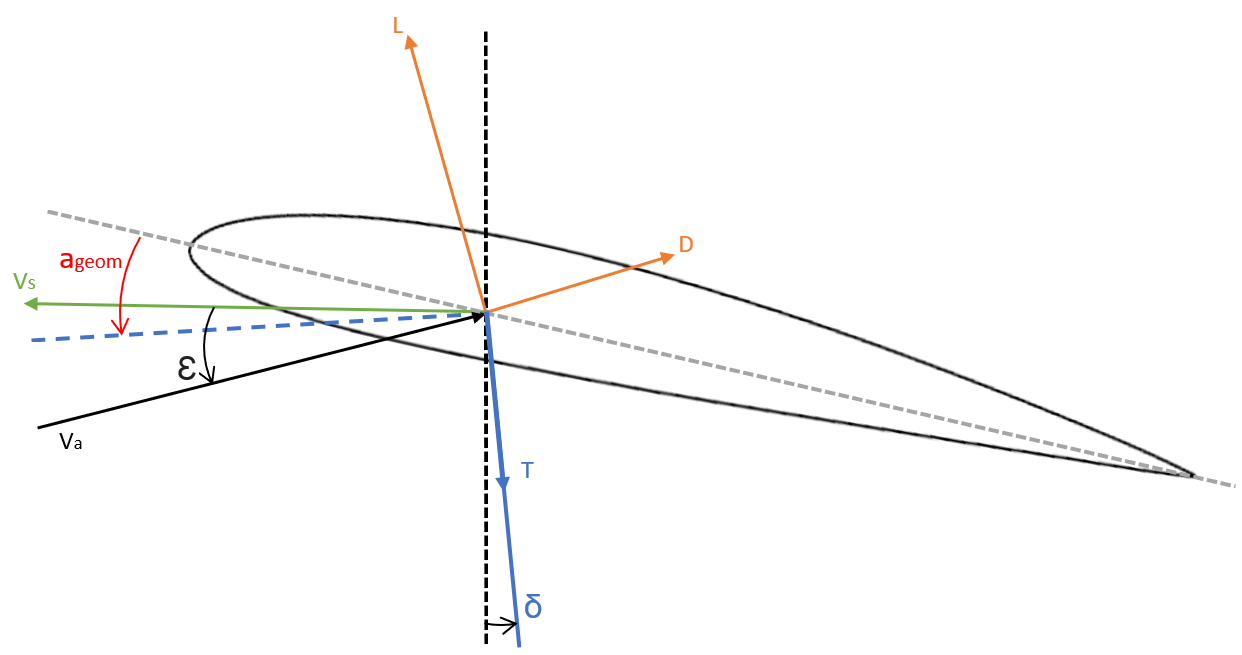
\includegraphics[width=1\textwidth]{figures/2D steady simulations/Angle calcul.png}
    \caption{Angle decomposition, taking into account the angle $\delta$ between the lines and the athlete}
    \label{fig:Angle decomposition, taking into account the angle $\delta$ between the lines and the athlete}
\end{figure}

\begin{figure}[H]
    \centering
    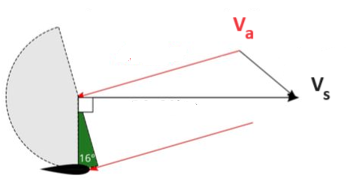
\includegraphics[width=0.6\textwidth]{figures/2D steady simulations/Ifremer work.png}
    \caption{The range of possible values for $\delta$ with an angle between the athlete's velocity vector and the apparent wind of 16°}
    \label{fig:The range of possible values for epsilon for an angle between the athlete's velocity vector and the apparent wind of 16°}
\end{figure}

 Consequently, the table \ref{tab:commonly_accepted_inlet_values} presents the generally acknowledged input parameters for a kite, as per the insights of kitesurfing experts and in consideration of Axel's race data :

 \begin{table}[H]
    \center
    \begin{tabular}{|l|l|l|}
        \hline
             & $\alpha_{i} ($°$) $ & $V_{a} (knots) $ \tabularnewline
        \hline
        Upwind & 0 - 5 & 30 - 35  \tabularnewline
        \hline
        Downwind & 7 - 14 & 18 - 23  \tabularnewline
        \hline
    \end{tabular}
    \caption{Commonly accepted inlet values}
    \label{tab:commonly_accepted_inlet_values}
\end{table}

%%%%%%%%%%%%%%%%%%%%%%%%%%%%%%%%%%%%%%%%%%%%%%%%%%%%%%%%%%%%%%%%%%%%%%%%%%%%%%%%
%%%%%%%%%%%%%%%%%%%%%%%%%%%%%%%%%%%% SECTION 4 %%%%%%%%%%%%%%%%%%%%%%%%%%%%%%%%%
%%%%%%%%%%%%%%%%%%%%%%%%%%%%%%%%%%%%%%%%%%%%%%%%%%%%%%%%%%%%%%%%%%%%%%%%%%%%%%%%

\section{XFLR5 - The plot of the aerodynamic polars}
\label{sec:Ch1.4}

%%%%%%%%%%%%%%%%%%%%%%%%%%%%%%%%%%%% SUBSECTION 1

\subsection{XFLR5}
\label{sub:Ch1.4.1}

XFLR5 is an analysis tool for airfoils, wings and planes operating at low Reynolds Numbers.

\begin{figure}[H]
    \centering
    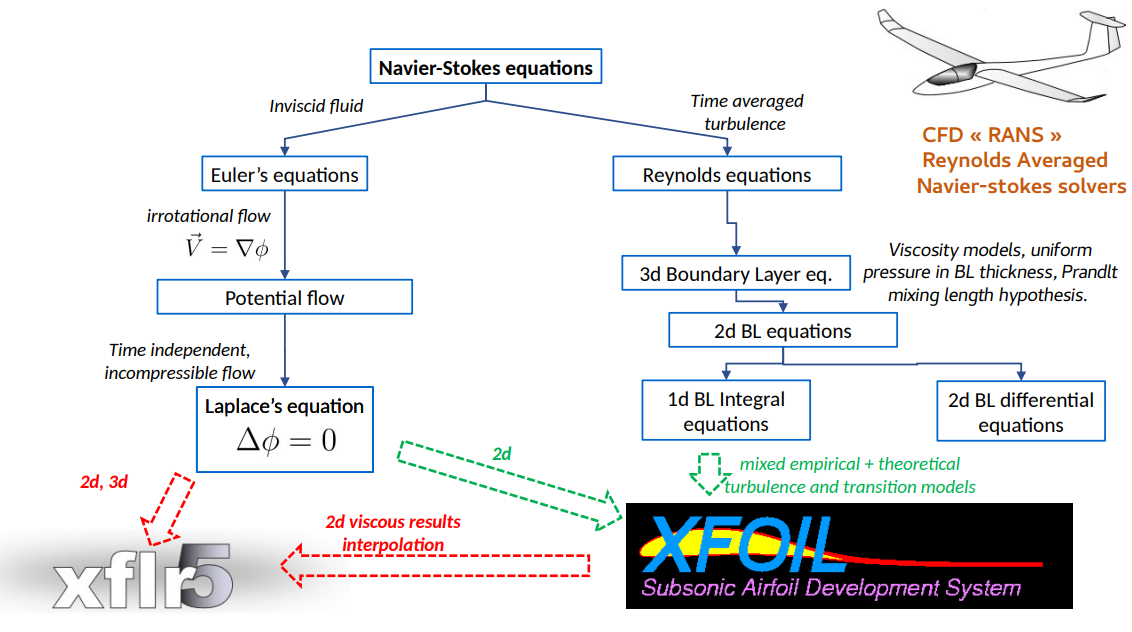
\includegraphics[width=1\linewidth]{figures/2D steady simulations/XFLR5 theory.png}
    \caption{XFLR5 theory diagram}
    \label{fig:XFLR5_theory_diagram}
\end{figure}

XFLR5 uses the "simultaneous" scheme, Developed by M. Drela and H. Youngren in the 1990s (XFOIL) at MIT, for solving the interactive boundary layer problem. It means that the inviscid and boundary layer equations are solved concurrently at each iteration\cite{XFLR5doc}.

In 2d, XFoil implements a full interactive boundary layer loop. However, XFOIL ultimately yields results that are accurate within the linear angle of attack range and below a Mach number of 0.4 but tends to overpredict lift and underpredict drag unless the flow is in the compressible regime. XFOIL cannot accurately model stall and post-stall conditions due to the nature of the solver\cite{XFOILlimits}.

%%%%%%%%%%%%%%%%%%%%%%%%%%%%%%%%%%%% SUBSECTION 2

\subsection{The polars}
\label{sub:Ch1.4.2}

Using XFLR5, I was able to plot the polars of the "R1 V4", the current Ozone kite, the "R1 V5", the next version of the R1 kites and the "VMG", the current kite of Flysurfer that was to be outperformed. 

The upwind polars have been plotted using a speed of 35 knots and a Reynolds number of $1,3e^{6}$

\begin{figure}[H]
\begin{subfigure}{0.5\textwidth}
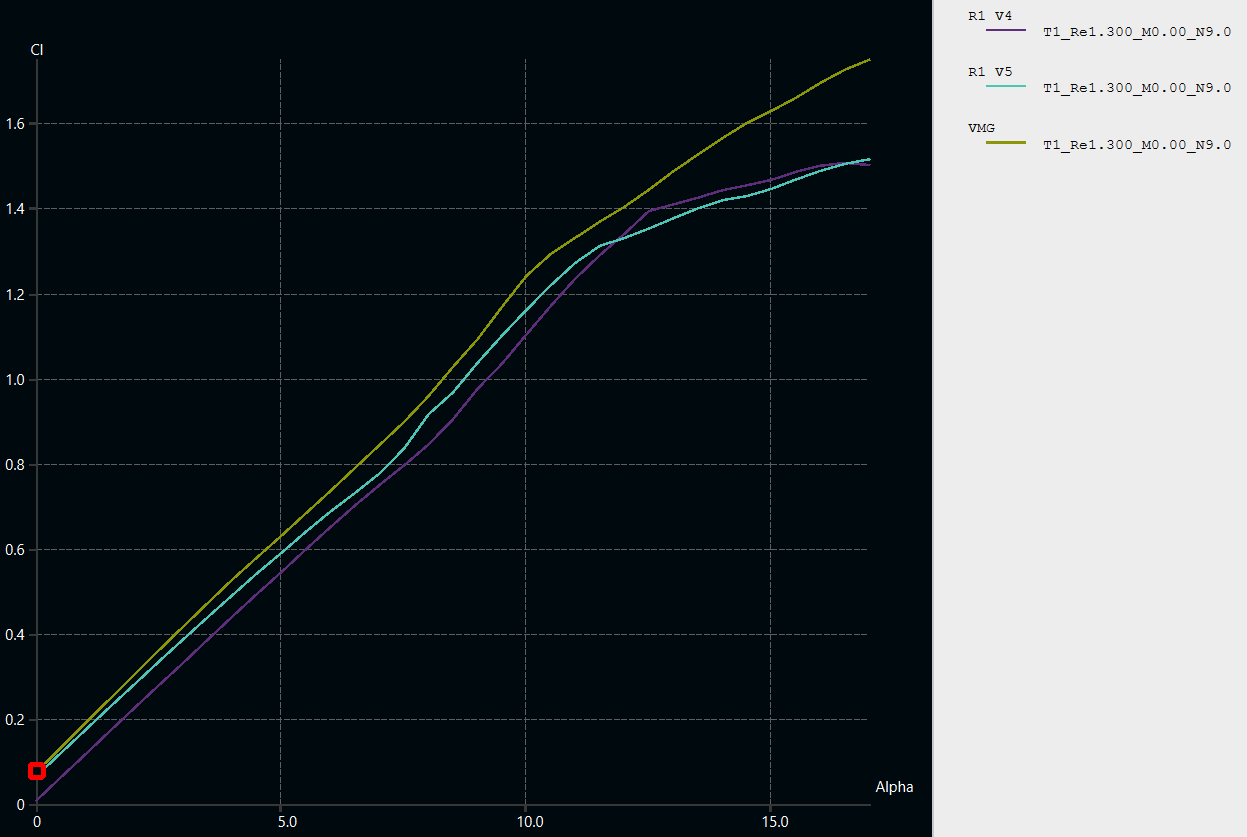
\includegraphics[width=1.\textwidth]{figures/2D steady simulations/xflr5/Cl upwind.png}
\caption{Plot of Cl upwind}
\label{fig:Plot_of_Cl_upwind}
\end{subfigure}
\begin{subfigure}{0.5\textwidth}
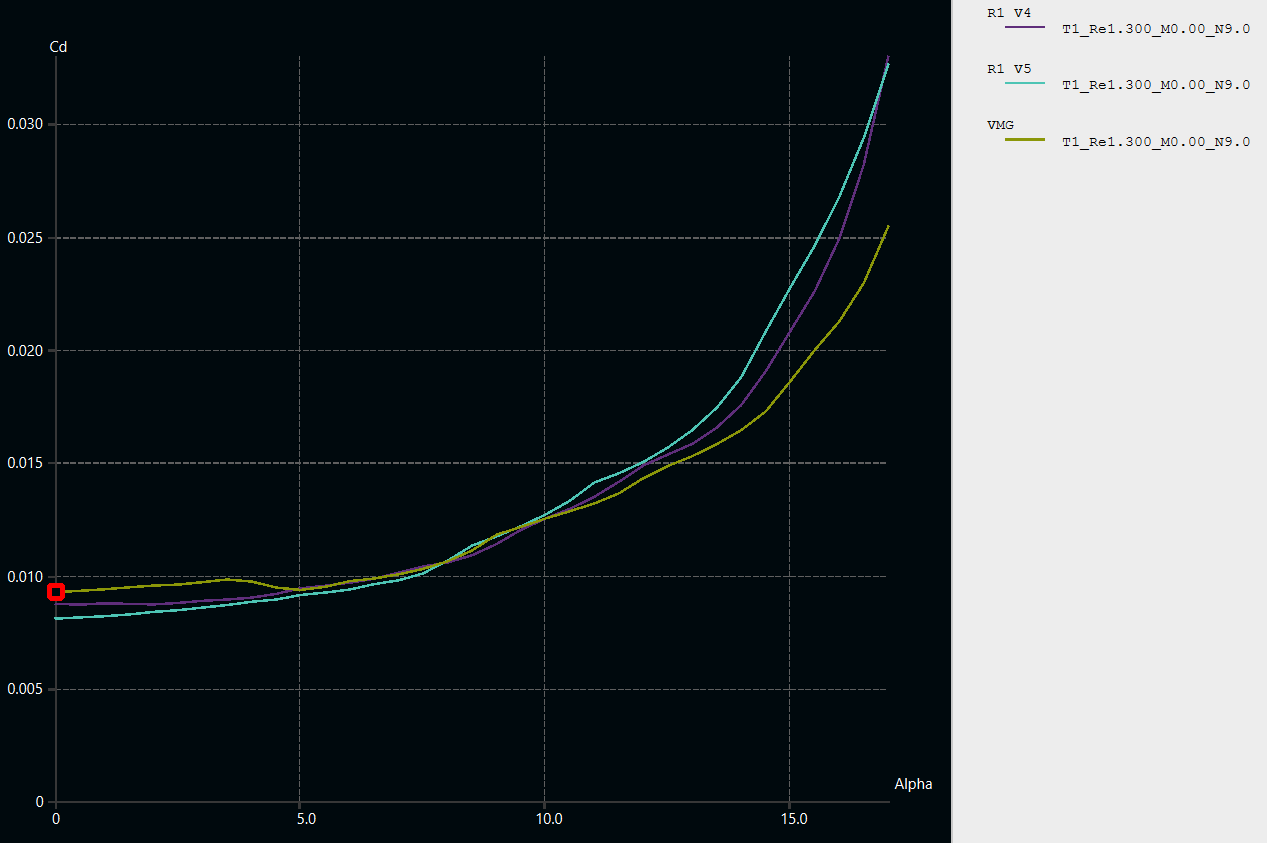
\includegraphics[width=01.\textwidth]{figures/2D steady simulations/xflr5/Cd upwind.png}
\caption{Plot of Cd upwind}
\label{fig:Plot_of_Cd_upwind}
\end{subfigure}
\caption{Upwind plots}
\label{fig:Upwind_plots}
\end{figure}

These polars are interesting for low angles of attack ( 0-5° according to \ref{tab:commonly_accepted_inlet_values} ) where one can see that the VMG and R1 V5 have a higher Cl than the R1 V4 and the R1 V5 has a lower Cd than the R1 V4 and the VMG. 

\begin{figure}[H]
    \centering
    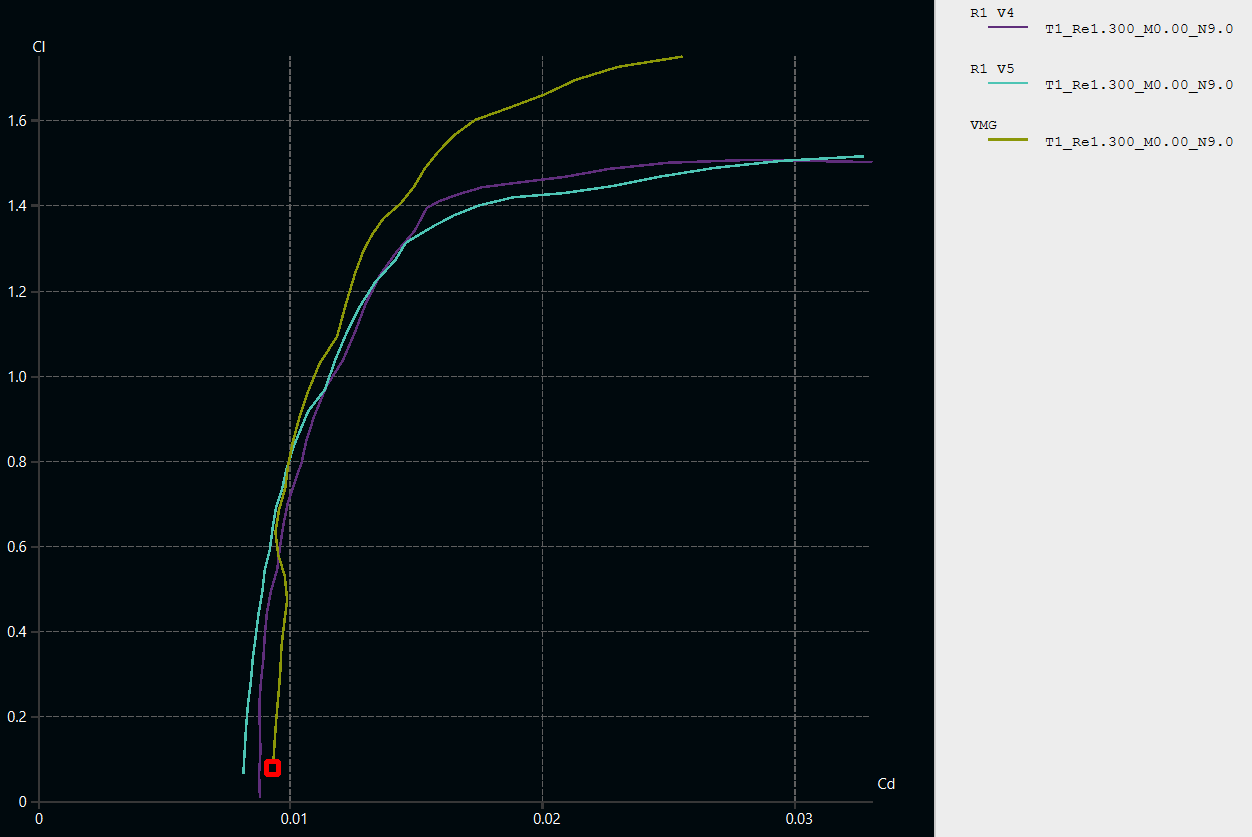
\includegraphics[width=0.5\textwidth]{figures/2D steady simulations/xflr5/Polar upwind.png}
    \caption{Upwind polars}
    \label{fig:Upwind_polars}
\end{figure}

Moreover, according to the team rider Axel Mazzela, "the R1 V4 is the one that does not fly enough to the edge of the wind window when the rider slacks (going upwind)". The lack of Cl (and therefore of finesse) in these conditions may be an explanation to that phenomena. 

However, these results need to be nuanced by the fact that at this stage the 3d effects are not taken into account.

For all the airfoils, the boundary layer transition from laminar to turbulent appears around 20$\%$ of the chord on the upper surface and 70$\%$ on the lower surface at an angle of attack of 5°. However, this result should be nuanced by the presence of seams along the leading edge of the kite, likely causing an earlier transition. Later in the internship, the transition had been deliberately induced to occur at the leading edge, and the comparison between the kites remained consistent.

%%
\vspace{1cm}
Then, the downwind polars have been plotted using a speed of 20 knots and a Reynolds number of $0,7e^{6}$

\begin{figure}[H]
\begin{subfigure}{0.5\textwidth}
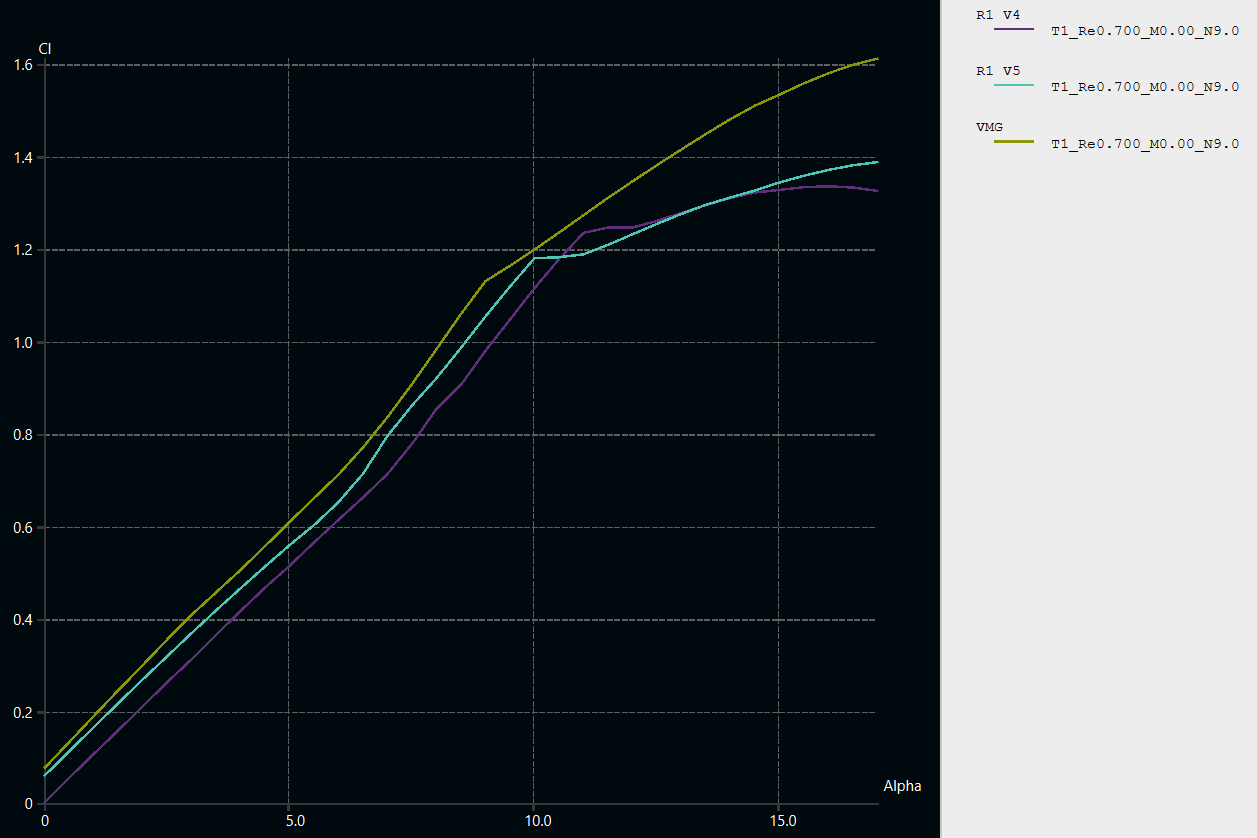
\includegraphics[width=1.\textwidth]{figures/2D steady simulations/xflr5/Cl downwind.png}
\caption{Plot of Cl downwind}
\label{fig:Plot_of_Cl_downwind}
\end{subfigure}
\begin{subfigure}{0.5\textwidth}
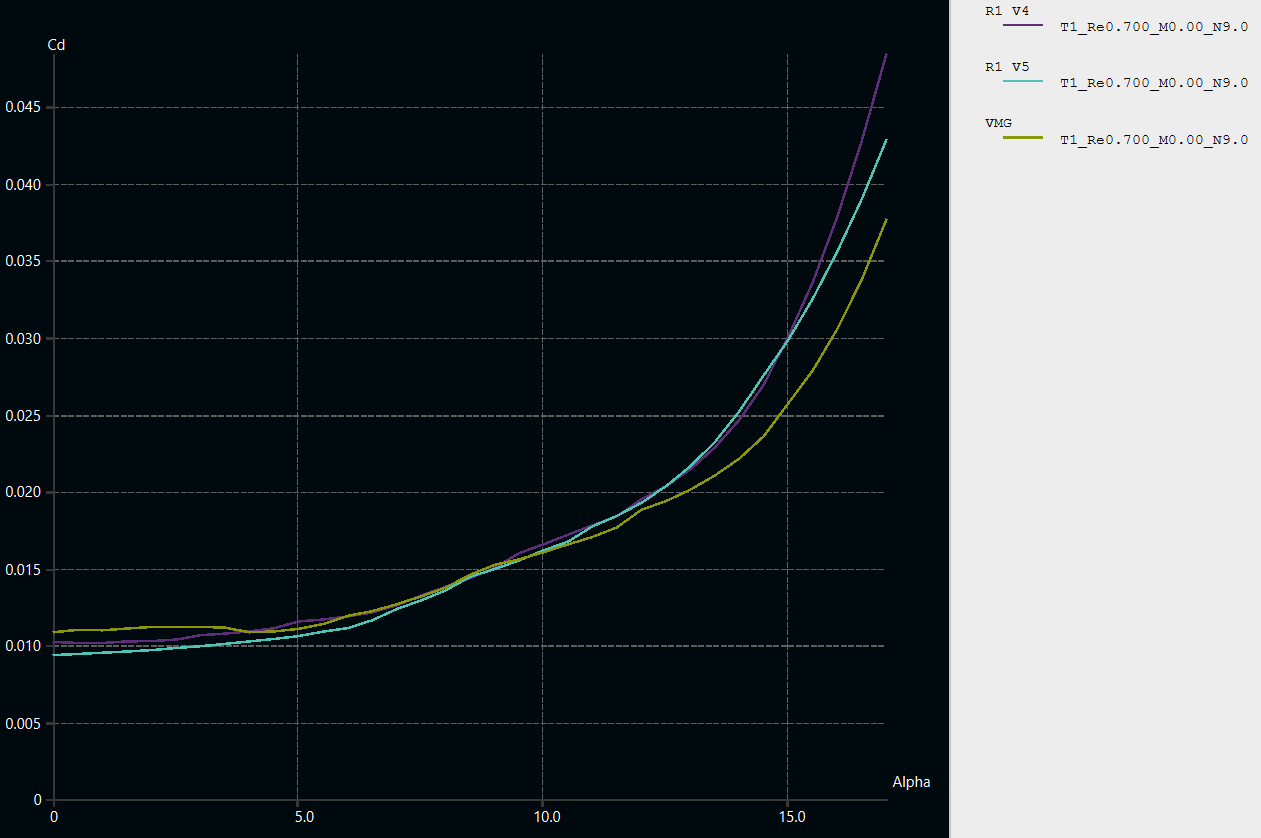
\includegraphics[width=1.\textwidth]{figures/2D steady simulations/xflr5/Cd Downwind.png}
\caption{Plot of Cd downwind}
\label{fig:Plot_of_Cd_downwind}
\end{subfigure}
\caption{Downwind plots}
\label{fig:Downwind_plots}
\end{figure}

These polars are interesting for higher angles of attack ( 7-14° according to \ref{tab:commonly_accepted_inlet_values} ) and need to be nuanced by the low reliability of XFLR5 at high angles of attack ( near the stall and post-stall ) \cite{XFOILlimits}. 


\begin{figure}[H]
    \centering
    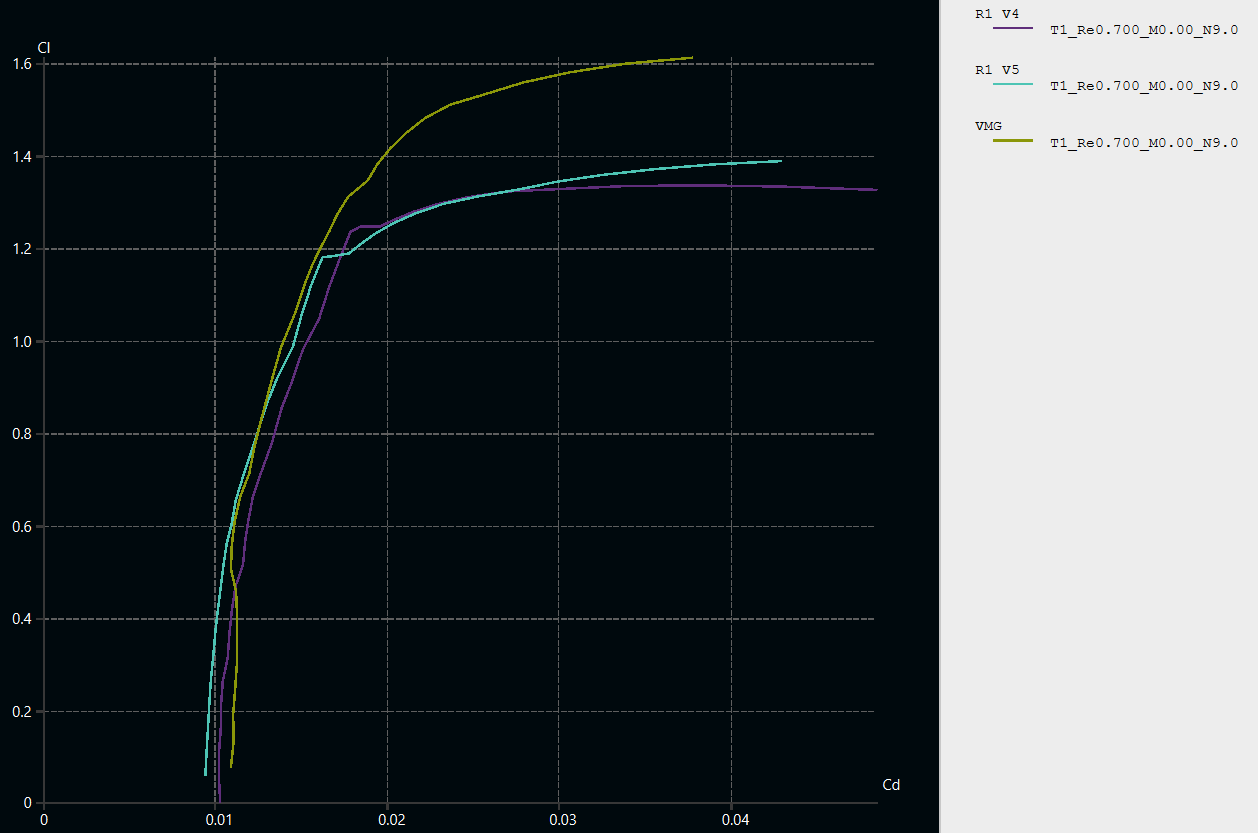
\includegraphics[width=0.5\textwidth]{figures/2D steady simulations/xflr5/Polar downwind.png}
    \caption{Downwind polars}
    \label{fig:Downwind_polars}
\end{figure}

We can see from these polars that the VMG has a higher Cl than the R1s and a lower Cd. 

According to Axel "the main issue with the R1 V5 is the low tether tension during this phase that can lead to a loose of tensions in the lines and its difficulty to fly forward when hauling the bar". 


Furthermore, comparing the R1 V4, which was only tested with three line sets, to the R1 V5 and the VMG, both of which were tested with only two line sets, proves challenging. In fact, Axel's observation suggests that with three lines, "the kite's shape is reinforced, and it catches the wind more quickly, resulting in a shorter transition time."

From this, it becomes apparent that the disparities in performance between the kites cannot be solely attributed to the airfoil design. Other factors, such as 3D effects and the number of lines, could provide a more comprehensive explanation for these results.

For all the airfoils, the boundary layer transition from laminar to turbulent appears around 16-19$\%$ of the chord on the upper surface and does not transit on the lower surface at an angle of attack of 10°. 

\textbf{From these results, and in connection with the experience of the team rider and both Ozone design teams (paraglider and kite), it appears that increasing the aerodynamic finesse of the R1 and enhancing lift in downwind conditions would enable them to surpass the VMG.}

%%%%%%%%%%%%%%%%%%%%%%%%%%%%%%%%%%%%%%%%%%%%%%%%%%%%%%%%%%%%%%%%%%%%%%%%%%%%%%%%
%%%%%%%%%%%%%%%%%%%%%%%%%%%%%%%%%%%% SECTION 5 %%%%%%%%%%%%%%%%%%%%%%%%%%%%%%%%%
%%%%%%%%%%%%%%%%%%%%%%%%%%%%%%%%%%%%%%%%%%%%%%%%%%%%%%%%%%%%%%%%%%%%%%%%%%%%%%%%

\section{The airfoil design}
\label{sec:Ch1.5}

Based on the preceding findings and in consultation with the Ozone design team, we generated the following Cp plot and conducted a comparative analysis of the foil designs in order to formulate our approach for the next airfoil prototype to be tested.

\begin{figure}[H]
\begin{subfigure}{0.5\textwidth}
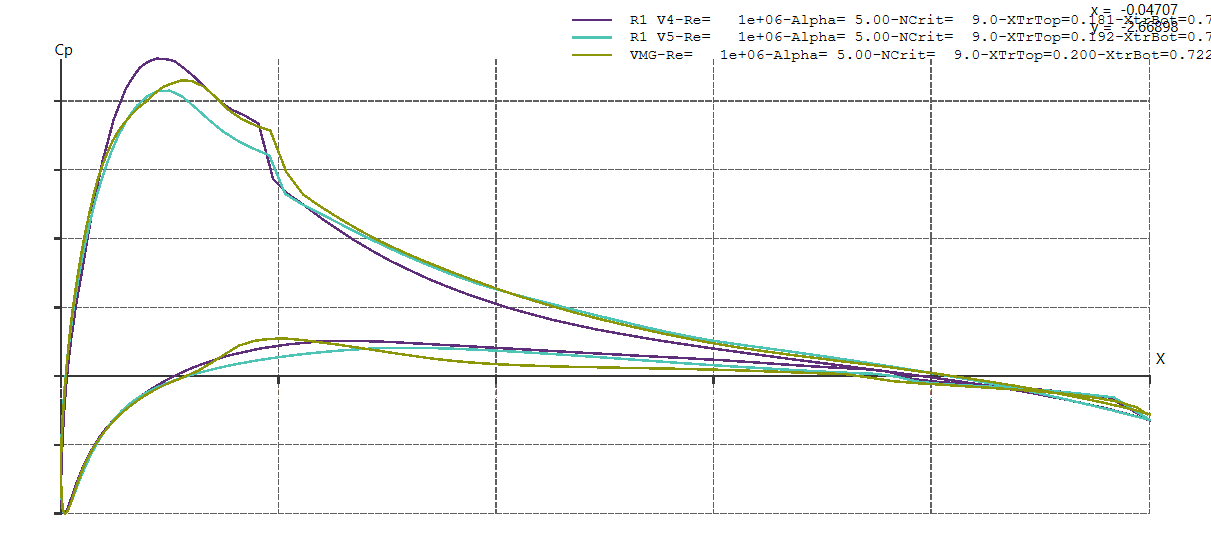
\includegraphics[width=1\textwidth]{figures/2D steady simulations/airfoil design/cp upwind 5deg.png}
\caption{Plot of Cp upwind at 5°}
\label{fig:Plot_of_Cp_upwind}
\end{subfigure}
\begin{subfigure}{0.5\textwidth}
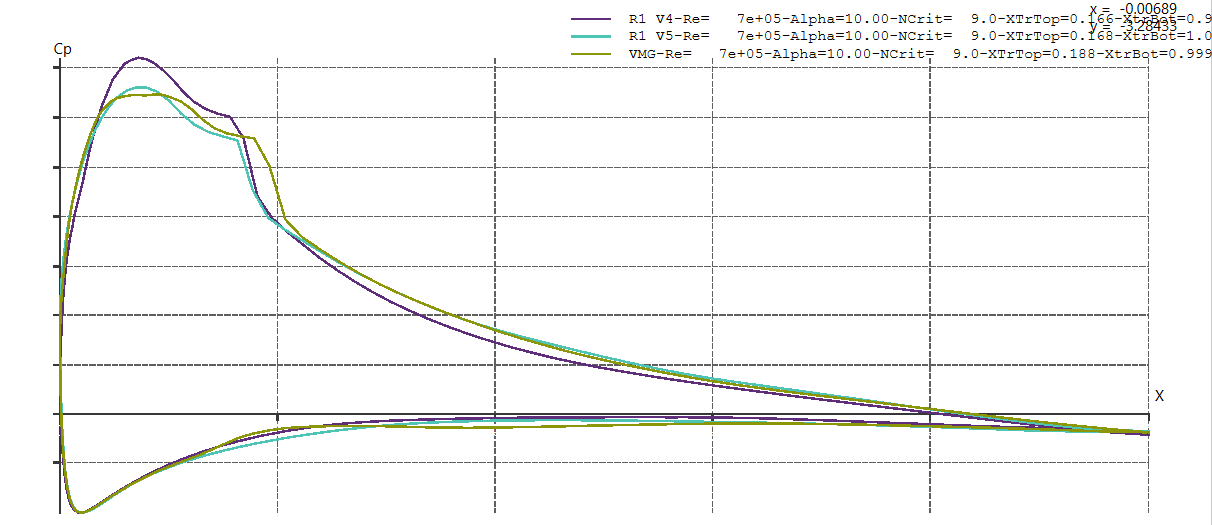
\includegraphics[width=1\textwidth]{figures/2D steady simulations/airfoil design/cp downwind 10deg.png}
\caption{Plot of Cp downwind at 10°}
\label{fig:Plot_of_Cp_downwind}
\end{subfigure}
\caption{Cp plots}
\label{fig:Cp_plots}
\end{figure}

We can see in the Cp plots that all kites have a peak of Cp on the upper surface near 10$\%$ of the chord then a boundary layer transition near 20$\%$ of the chord. However, if the R1 V4 has the highest peak, it also have a higher Cp on the lower surface which leads to a lower C$_{L}$. The R1 V5 has a lower Cp peak on the upper surface than the R1 V4 but also a lower Cp on the lower surface.

The VMG upper surface seems to be a good compromise between the three different Cp plot as its peak is lower than the R1 V4 but its turbulent part is higher.

However, the R1s' lower surfaces seem to be better than the VMG because they lead to mostly lower and smoother Cp plot.

\vspace{1cm}

If we consider the airfoils, we can see that the VMG lower surface reaches its lowest point earlier than the other airfoils which may lead too a smoother interaction between the intrados and extrados flows at the trailing edge (because its recompression zone is larger).

\begin{figure}[H]
    \centering
    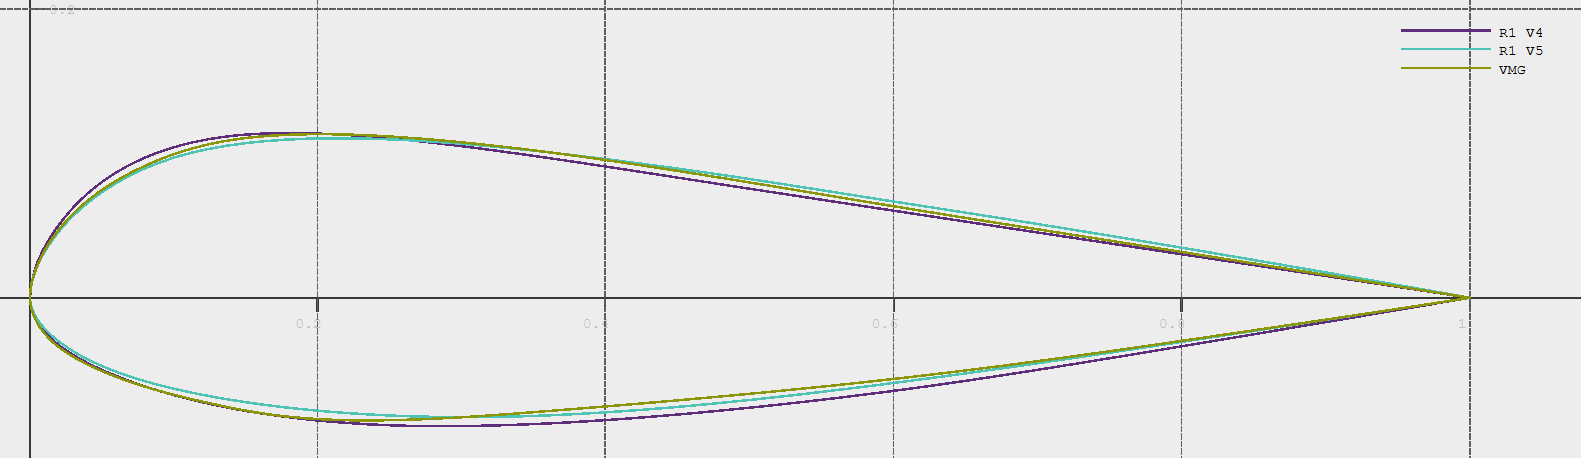
\includegraphics[width=0.8\textwidth]{figures/2D steady simulations/airfoil design/foils design.png}
    \caption{The 3 different airfoil designs}
    \label{fig:The_3_different_airfoil_designs}
\end{figure}

As a result, with the help of Rob Whittall, product designer, co-owner and co-founder of Ozone, we designed a new airfoil making the lower surface of the R1 V5 "smoother" and changing the VMG upper surface making its leading edge "rounder". The resulting airfoil was named "R1 V5 Satori 3". 

\begin{figure}[H]
\begin{subfigure}{1\linewidth}
\centering
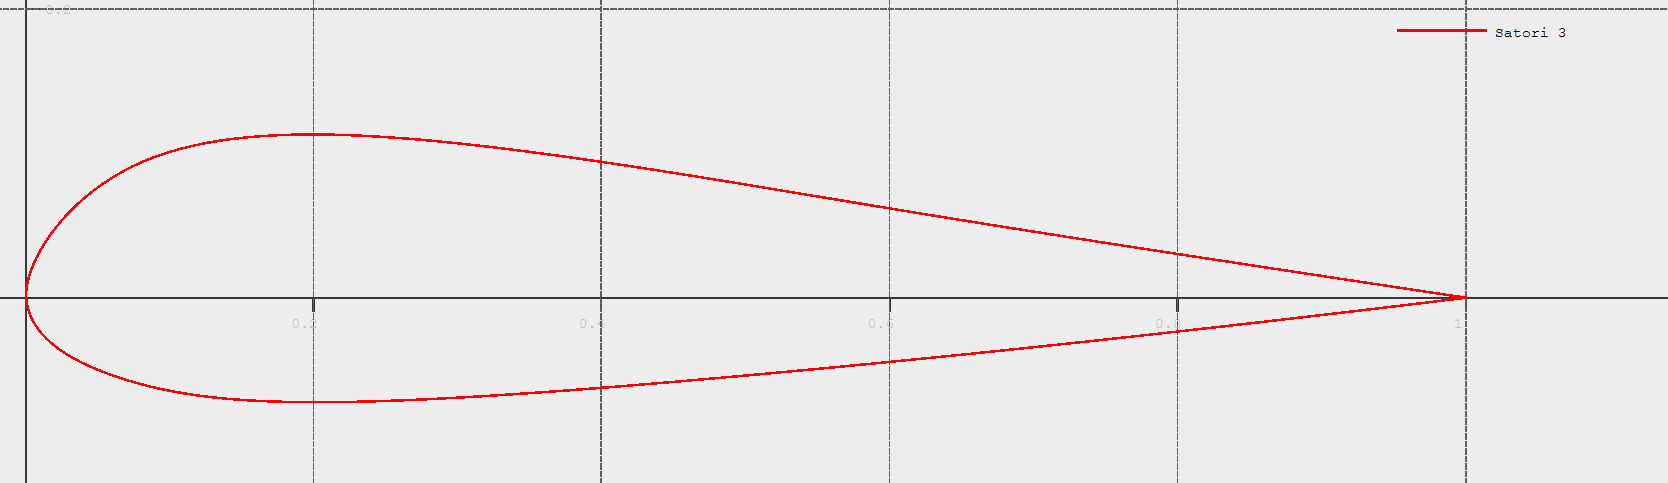
\includegraphics[width=0.9\textwidth]{figures/2D steady simulations/airfoil design/satori 3.png}
\caption{The R1 V5 Satori 3 airfoil}
\label{fig:The_R1_V5_Satori_3_airfoil}
\end{subfigure}
\centering
\begin{subfigure}{0.9\linewidth}
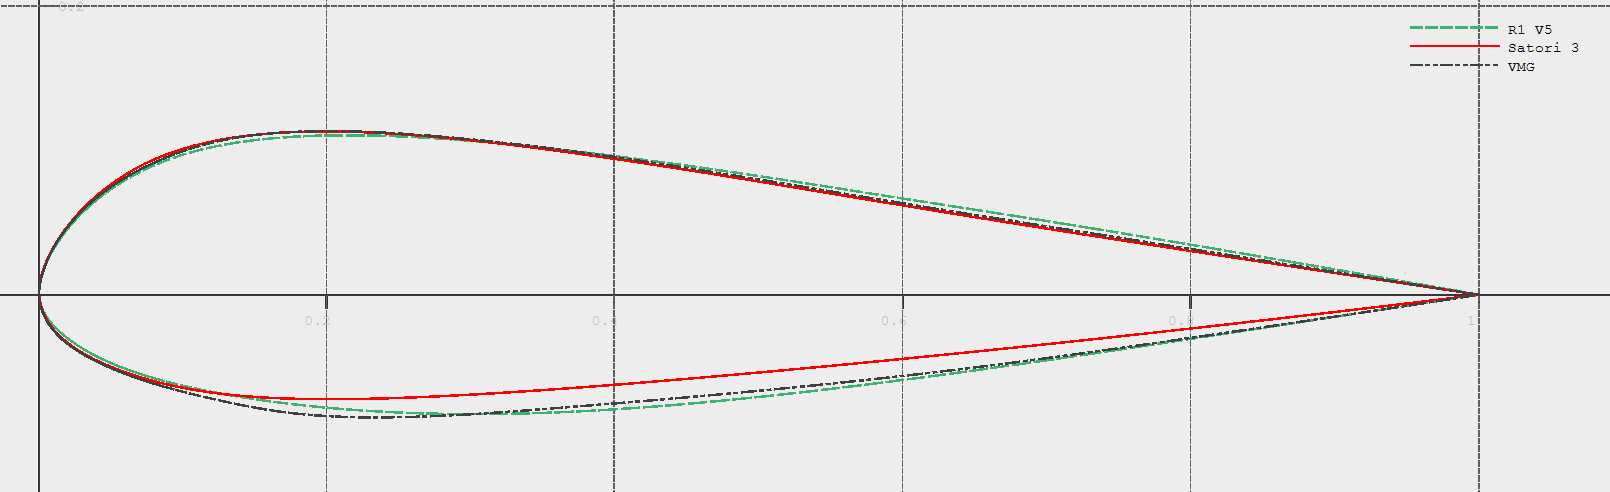
\includegraphics[width=1.\textwidth]{figures/2D steady simulations/airfoil design/satori 3, R1V5 and VMG.png}
\caption{The R1 V5 Satori 3, R1 V5 and VMG airfoils}
\label{fig:The_R1_V5_Satori_3,_R1_V5_and_VMG_airfoils}
\end{subfigure}
\caption{Cp plots}
\label{fig:Comparison between different airfoil designs}
\end{figure}

The following graphs \ref{fig:Cd_Cl_plot_of_the_VMG_and_R1_V5_Satori_3} and \ref{fig:Polar_of_the_VMG_and_R1_V5_Satori_3} show that the R1 V5 Satori 3 has a higher Cl, lower Cd and, as a result, a higher finesse upwind at 5° and downwind at 10°. 

\begin{figure}[H]
\begin{subfigure}{0.5\textwidth}
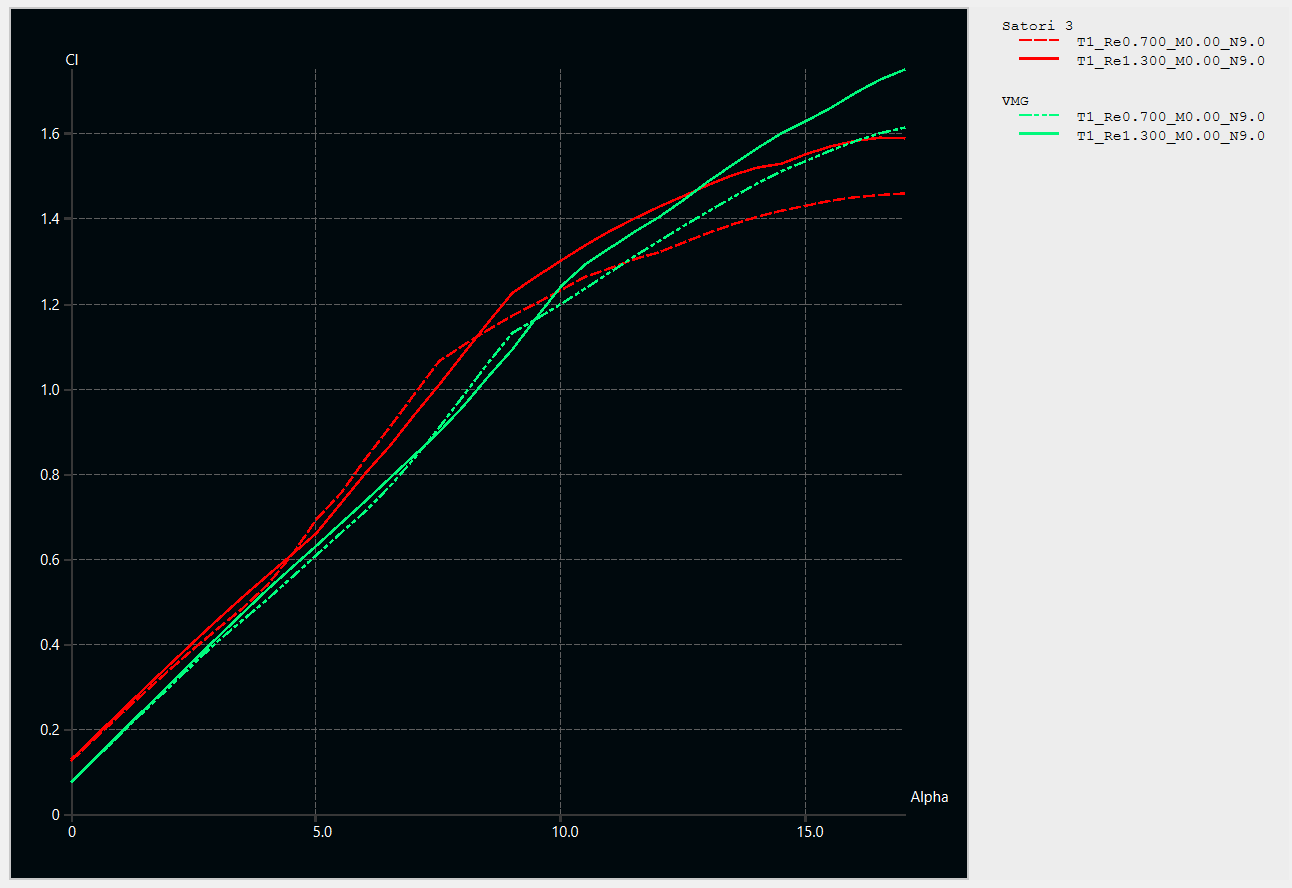
\includegraphics[width=1\textwidth]{figures/2D steady simulations/xflr5/Cl vmg sat3.png}
\caption{Cl plot}
\label{fig:Cl_plot_of_the_VMG_and_R1_V5_Satori_3}
\end{subfigure}
\begin{subfigure}{0.5\textwidth}
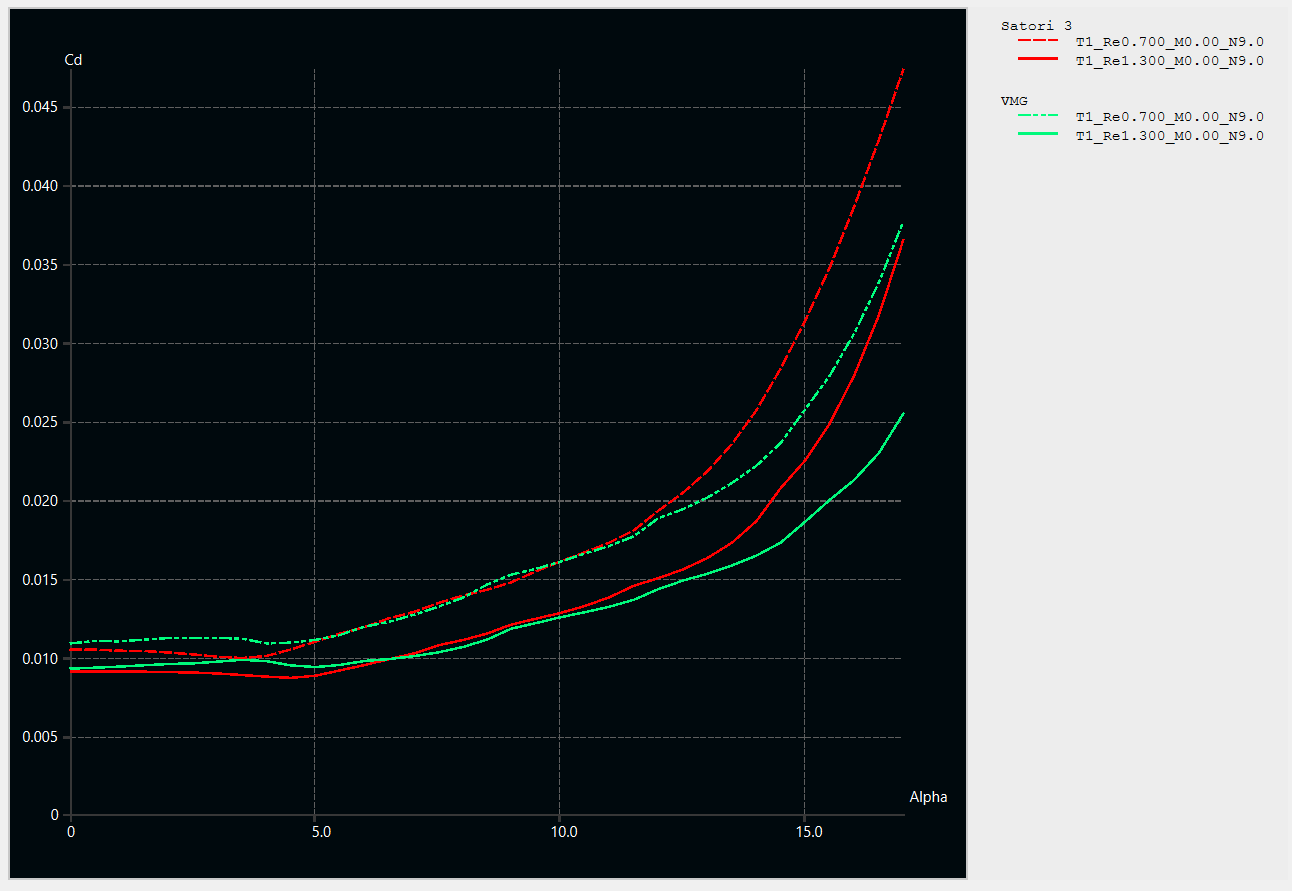
\includegraphics[width=1\textwidth]{figures/2D steady simulations/xflr5/Cd vmg sat3.png}
\caption{Cd}
\label{fig:Cd_plot_of_the_VMG_and_R1_V5_Satori_3}
\end{subfigure}
\caption{Cd $\&$ Cl plots (VMG and R1 V5 Satori 3)}
\label{fig:Cd_Cl_plot_of_the_VMG_and_R1_V5_Satori_3}
\end{figure}

\begin{figure}[H]
    \centering
    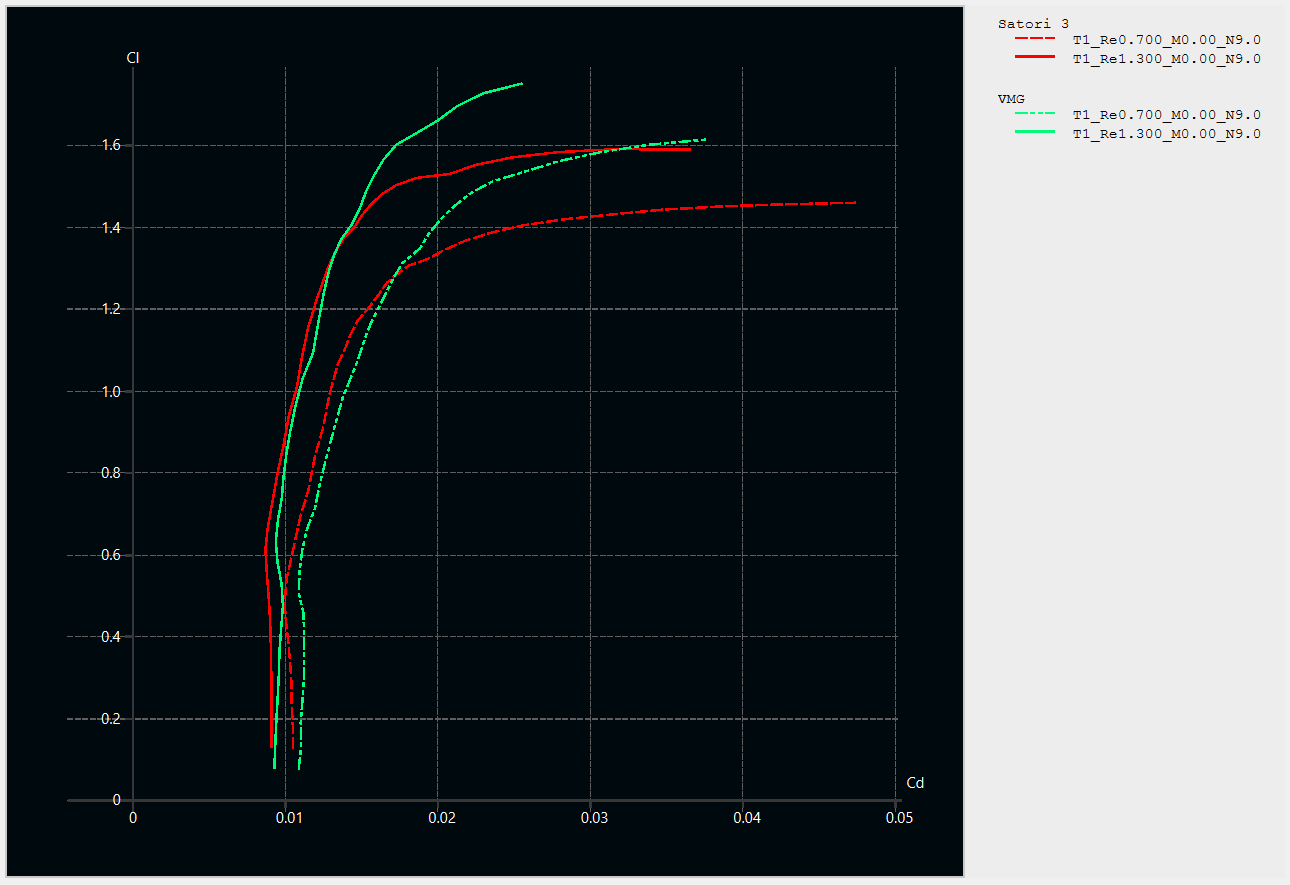
\includegraphics[width=0.75\textwidth]{figures/2D steady simulations/xflr5/polar vmg sato3.png}
    \caption{Polars (VMG and R1 V5 Satori 3)}
    \label{fig:Polar_of_the_VMG_and_R1_V5_Satori_3}
\end{figure}

Moreover, we can see on the figure \ref{fig:Cp_plots_of_VMG_and_R1_V5_Satori_3} that the objectives in term of Cp plot have been reached. 

\begin{figure}[H]
    \begin{subfigure}{0.5\linewidth}
    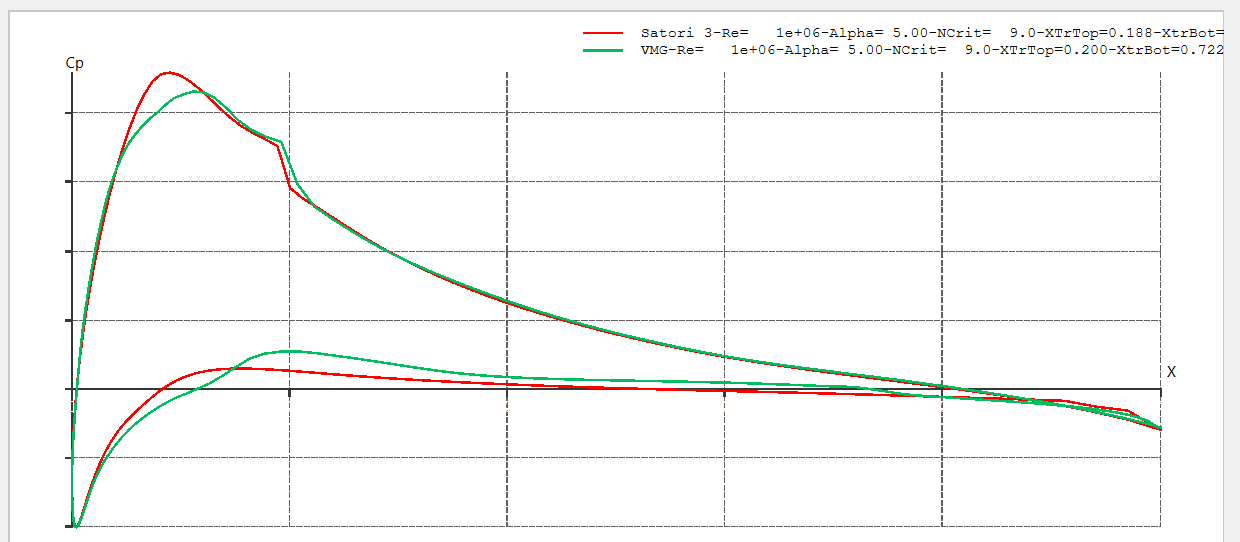
\includegraphics[width=1.\linewidth]{figures/2D steady simulations/airfoil design/cp upwind 5deg vmg sato3.png}
    \caption{Cp plot upwind at 5°}
    \label{fig:Cp_plot_upwind_at_5°}
    \end{subfigure}
    \begin{subfigure}{0.5\linewidth}
    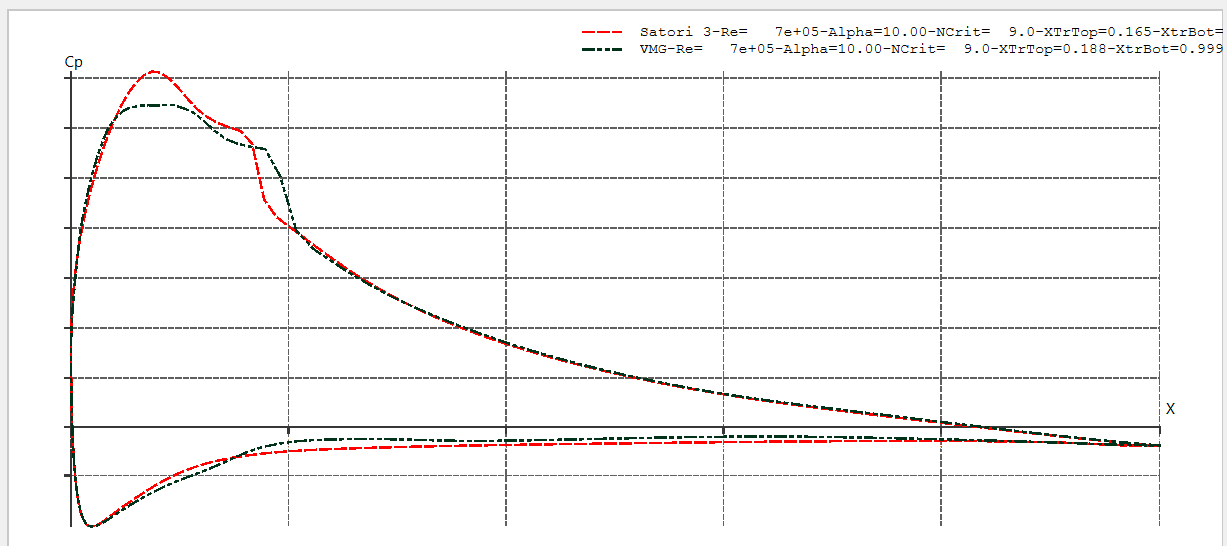
\includegraphics[width=1.\linewidth]{figures/2D steady simulations/airfoil design/cp downwind 10deg vmg sato3.png}
    \caption{Cp plot downwind at 10°}
    \label{fig:Cp_plot_downwind_at_10°}
    \end{subfigure}
    \caption{Cp plots of VMG and R1 V5 Satori 3}
\label{fig:Cp_plots_of_VMG_and_R1_V5_Satori_3}
\end{figure}

%%%%%%%%%%%%%%%%%%%%%%%%%%%%%%%%%%%%%%%%%%%%%%%%%%%%%%%%%%%%%%%%%%%%%%%%%%%%%%%%
%%%%%%%%%%%%%%%%%%%%%%%%%%%%%%%%%%%% SECTION 6 %%%%%%%%%%%%%%%%%%%%%%%%%%%%%%%%%
%%%%%%%%%%%%%%%%%%%%%%%%%%%%%%%%%%%%%%%%%%%%%%%%%%%%%%%%%%%%%%%%%%%%%%%%%%%%%%%%

\section{FLUENT - The 2D steady simulations}
\label{sec:Ch1.6}

%%%%%%%%%%%%%%%%%%%%%%%%%%%%%%%%%%%% SUBSECTION 1

\subsection{The spatial convergence}
\label{sub:Ch1.6.1}

We conducted comparisons using ANSYS FLUENT to refine the results. The objective was to provide Ozone with a more precise comprehension of the flow characteristics around their airfoils and accurate aerodynamic coefficients, particularly in the vicinity of the stall, where XFLR5 is recognized to be less reliable. 

The meshing was done using the FLUENT meshing software. For a flow speed from 20 to 35 knots and $y{+} = 1$, $\delta y = 3.4e^{-5}$ to $2e^{-5}$. These value were respected.

Furthermore, spatial merging has been confirmed for all airfoil designs. To illustrate, consider the R1 V5 Satori 3, which yielded the following results: 

\begin{table}[H]
    \center
    \begin{tabular}{|l|l|l|l|}
        \hline
        number of elements & 138653 & 200150 & 288180 \tabularnewline
        \hline
        CL & 0,1276 & 0,1272 & 0,1258  \tabularnewline
        \hline
        CD & 0,0124 & 0,01245 & 0,0124  \tabularnewline
        \hline
        Finesse & 10,2903 & 10,2169 & 10,1452  \tabularnewline
        \hline
    \end{tabular}
    \caption{R1 V5 Satori 3 results at O° and 30 knots}
    \label{tab:R1_V5_results_at_O°_and_35_knots}
\end{table}

Then, using the Richardson interpolation method \cite{RichardsonInterpolation}:

\begin{equation}
\left \{
   \begin{array}{r c l}
      p  & = & \frac{1}{ln(r)} \frac{ln(m_{3}-m_{2})}{ln(m_{2}-m_{1})} \\
      m^{*}   & = & \frac{m_{3}-m_{2}r^{p}}{1-r^{p}} \\
   \end{array}
   \right .
   \label{Richardson_interpolation}
\end{equation}
(with $m_{i}$ the results obtained for meshes with element sizes in a ratio r, $m^{*}$ the asymptotic value and p the merging order)

We obtain : 

\begin{table}[H]
    \center
    \begin{tabular}{|l|l|l|l|}
        \hline
           & p & Asymptotic value & Required accuracy \tabularnewline
        \hline
        CL & 2,30 &  0,1247 & $e^{-2}$ \tabularnewline
        \hline
        CD & 2,73 & 0,0124 & $e^{-3}$ \tabularnewline
        \hline
        Finesse & 2,76 & 10,1452 &  $e^{0}$ \tabularnewline
        \hline
    \end{tabular}
    \caption{R1 V5 asymptotic results at O° and 30 knots}
    \label{tab:R1_V5_asymptotic_results_at_O°_and_35_knots}
\end{table}

\begin{figure}[H]
    \centering
    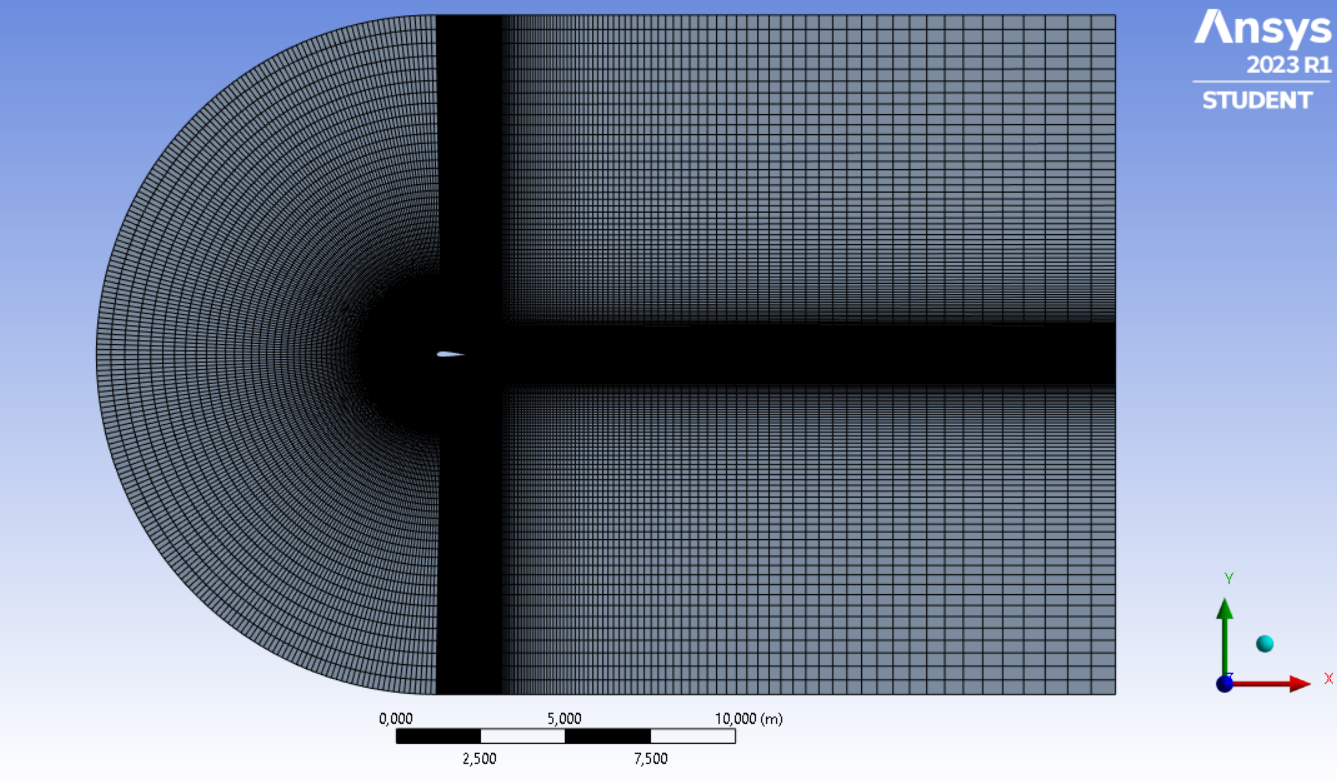
\includegraphics[width=1\textwidth]{figures/2D steady simulations/fluent/R1 V5 meshing.png}
    \caption{The global meshing under FLUENT}
    \label{fig:The global meshing}
\end{figure}

\begin{figure}[H]
    \centering
    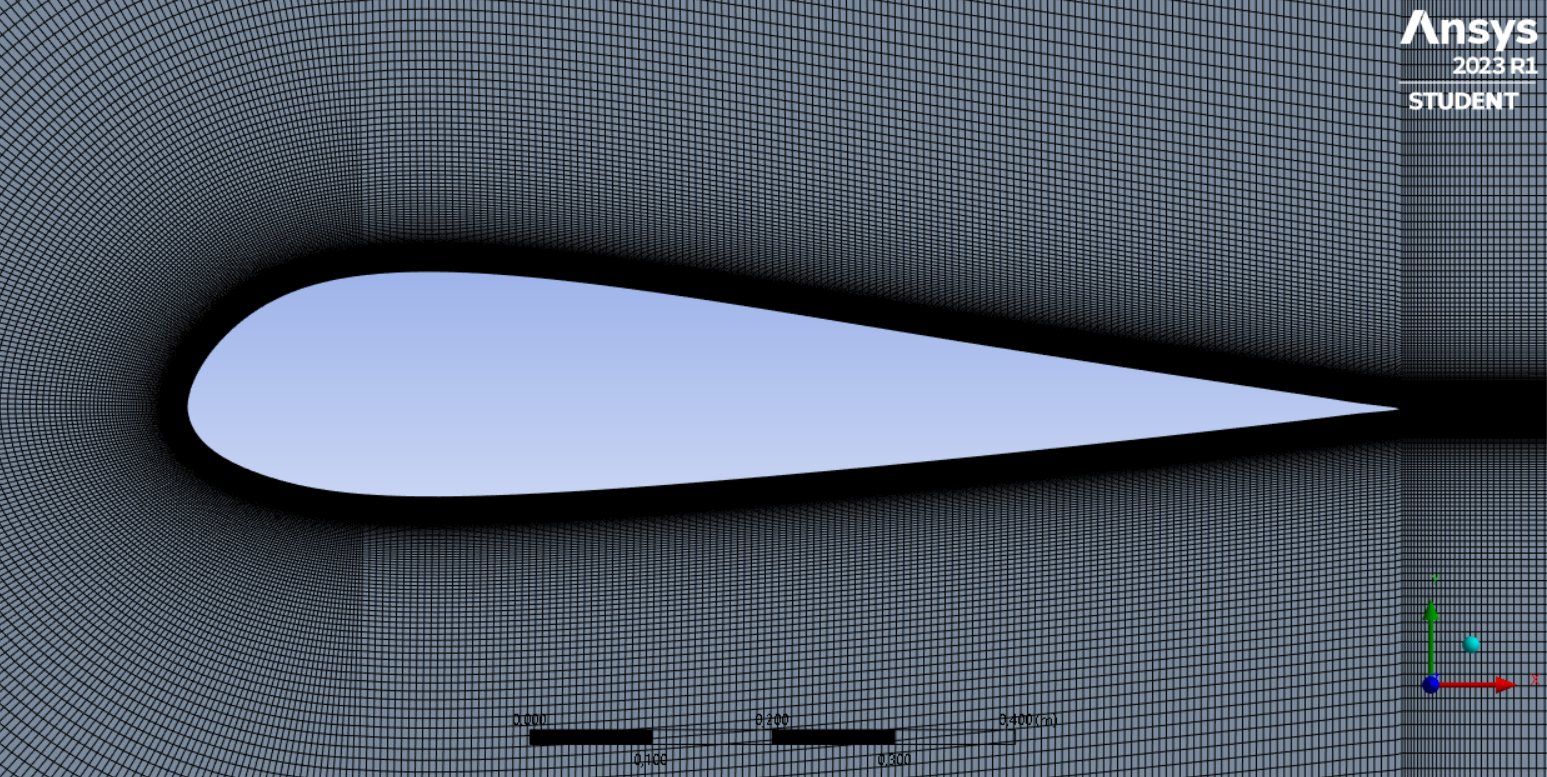
\includegraphics[width=0.75\textwidth]{figures/2D steady simulations/fluent/R1 V5 meshing zoom.png}
    \caption{Zoom on the airfoil}
    \label{fig:Zoom on the meshing}
\end{figure}


%%%%%%%%%%%%%%%%%%%%%%%%%%%%%%%%%%%% SUBSECTION 2

\subsection{The turbulence models}
\label{sub:Ch1.6.2}

FLUENT offers various turbulence models. 

Two models were tested to nuance the results :
\begin{itemize}
    \item \textbf{Spalart-Allmaras : } \\
    it is the only example of a transport equation model for $\nu_{t}$ used in the industry. This model is widely used in aeronautics for various reasons: It is easy to numerically integrate, for attached flows, it produces results as good as zero-equation models, and for separated flows, it provides a much better description of the velocity field than zero-equation models. However, this model is too simple (a single equation) to be valid for a wide range of flows \cite{turbulentmodels}.
    \item \textbf{k-$\omega$ SST : } \\
    The idea is to formulate a set of equations that converge towards the k-$\omega$ model near the wall and towards the k-$\epsilon$ model far from the walls. This model has been successfully applied in many configurations. It is currently one of the preferred models in the aerospace industry.
    k-$\omega$ provides better results than the standard k-$\epsilon$ and model in adverse pressure gradient situations, allowing for a more accurate prediction of separation points. The k-$\epsilon$ and k-$\omega$ models use two scales, not just one, so the aim is to overcome the limitations of the Spalart-Allmaras model.
    However, this first-order linear model comes with several assumptions :
    \begin{itemize}
        \item instantaneity, where the deformation and turbulence history have no influence
        \item locality, where turbulence is influenced only by its immediate surroundings.
        \item materially simple environment
        \item linearity of the behavior law
    \end{itemize}
    It is understood, then, that first-order linear models cannot work in all situations \cite{turbulentmodels}.
\end{itemize}

The figures \ref{fig:polars comparison between turbulence models on the R1 V5 Satori 3} and \ref{fig:Finesse relative error between turbulence models} compares the R1 V5 Satori 3 finesse plot at 35 knots with the two turbulence models. While the k-$\omega$ SST model is designed to provide more precise outcomes compared to the Spalart-Allmaras model, it introduces an elevated computational expense and an added difficulty in attaining spatial convergence. This is in contrast to the Spalart-Allmaras model, which generally converges toward a solution (that has spatially converged). Additionally, at low angles of attack, both models produce similar outcomes. It is only when encountering high angles of attack that noticeable disparities in results arise, reaching approximately 15\% divergence.

\begin{figure}[H]
    \centering
    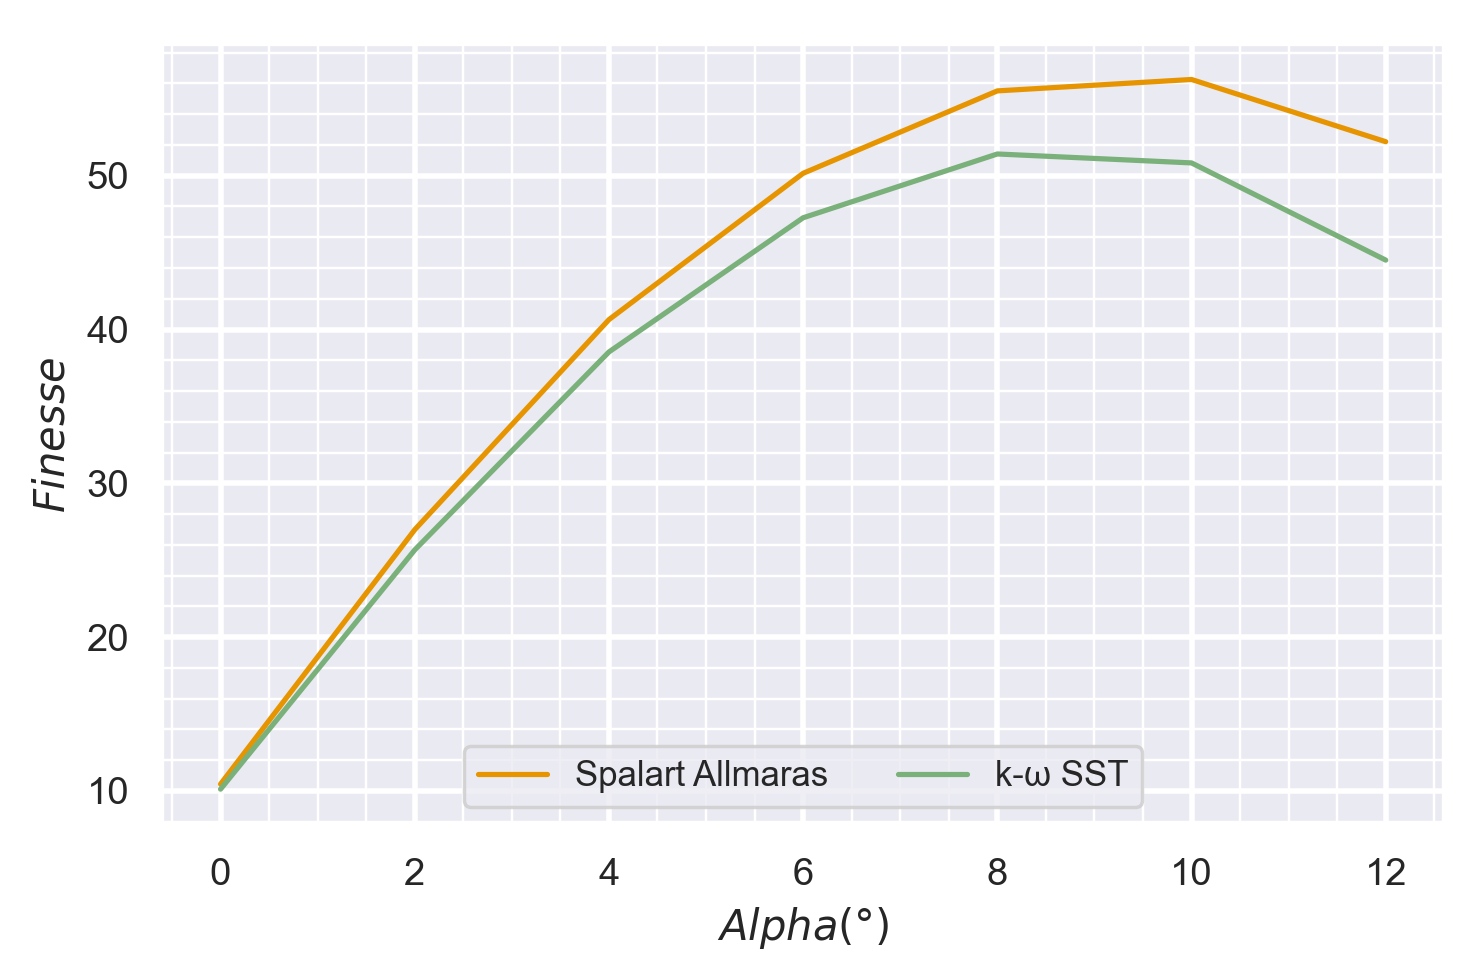
\includegraphics[width=0.75\linewidth]{figures/2D steady simulations/fluent/R1V5Satori3 Spalart Allmaras VS KWSST.png}
    \caption{finesse against alpha}
    \label{fig:polars comparison between turbulence models on the R1 V5 Satori 3}
\end{figure}

\begin{figure}[H]
    \centering
    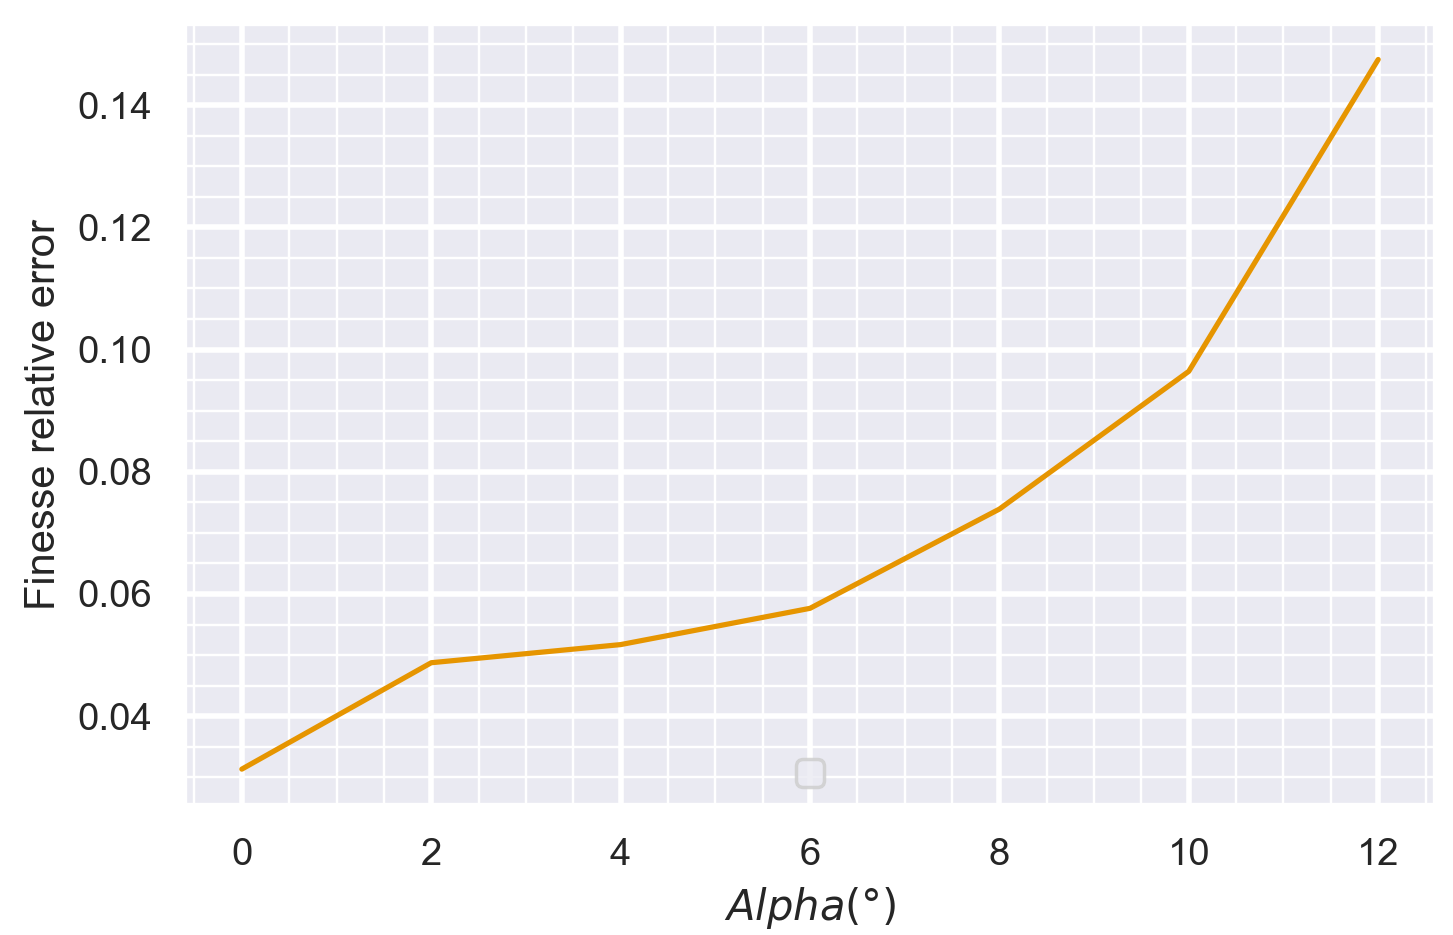
\includegraphics[width=0.75\linewidth]{figures/2D steady simulations/fluent/finesse relative error turbulence model.png}
    \caption{Finesse relative error against alpha}
    \label{fig:Finesse relative error between turbulence models}
\end{figure}

As a result, knowing the level of accuracy Ozone was looking for and the computational cost we could afford, \textbf{the Spalart-Allmaras model is the one we chose for our simulations}. 

\textbf{It's important to note that Ozone Kitesurf didn't seek highly precise results. Their primary objective was to gain insights into enhancing their existing airfoil while obtaining results that align with overall trends. Additionally, due to the computational limitations of my computer and the recognized influences of 3D effects, unsteadiness and fluid structure interactions, the pursuit of more precise results became less appealing.}

%%%%%%%%%%%%%%%%%%%%%%%%%%%%%%%%%%%% SUBSECTION 3

\subsection{The results}
\label{sub:Ch1.6.3}

The following figure \ref{fig:The R1 V5 meshing under FLUENT} shows the finesse plots for the R1 V5, R1 V5 Satori 3 and the VMG at 15 knots, the downwind conditions, and 35 knots, the upwind conditions. 

\begin{figure}[H]
    \begin{subfigure}{0.5\textwidth}
    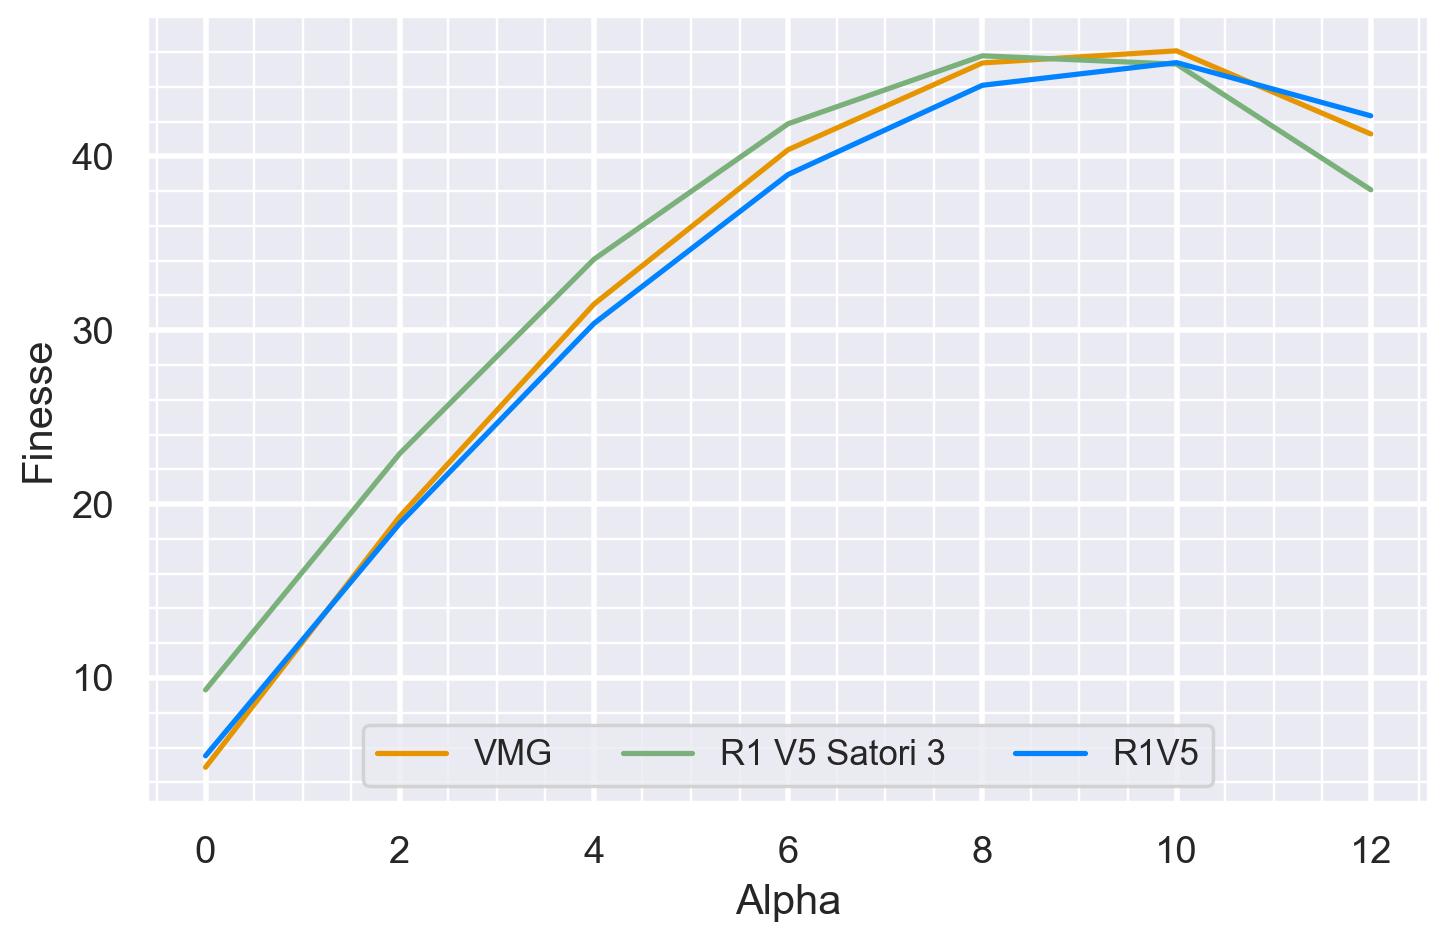
\includegraphics[width=1\textwidth]{figures/2D steady simulations/fluent/finesse VMG SAT3 R1V5 15kts FLUENT.png}
    \caption{15 knots}
    \label{fig:15 knots}
    \end{subfigure}
    \begin{subfigure}{0.5\textwidth}
    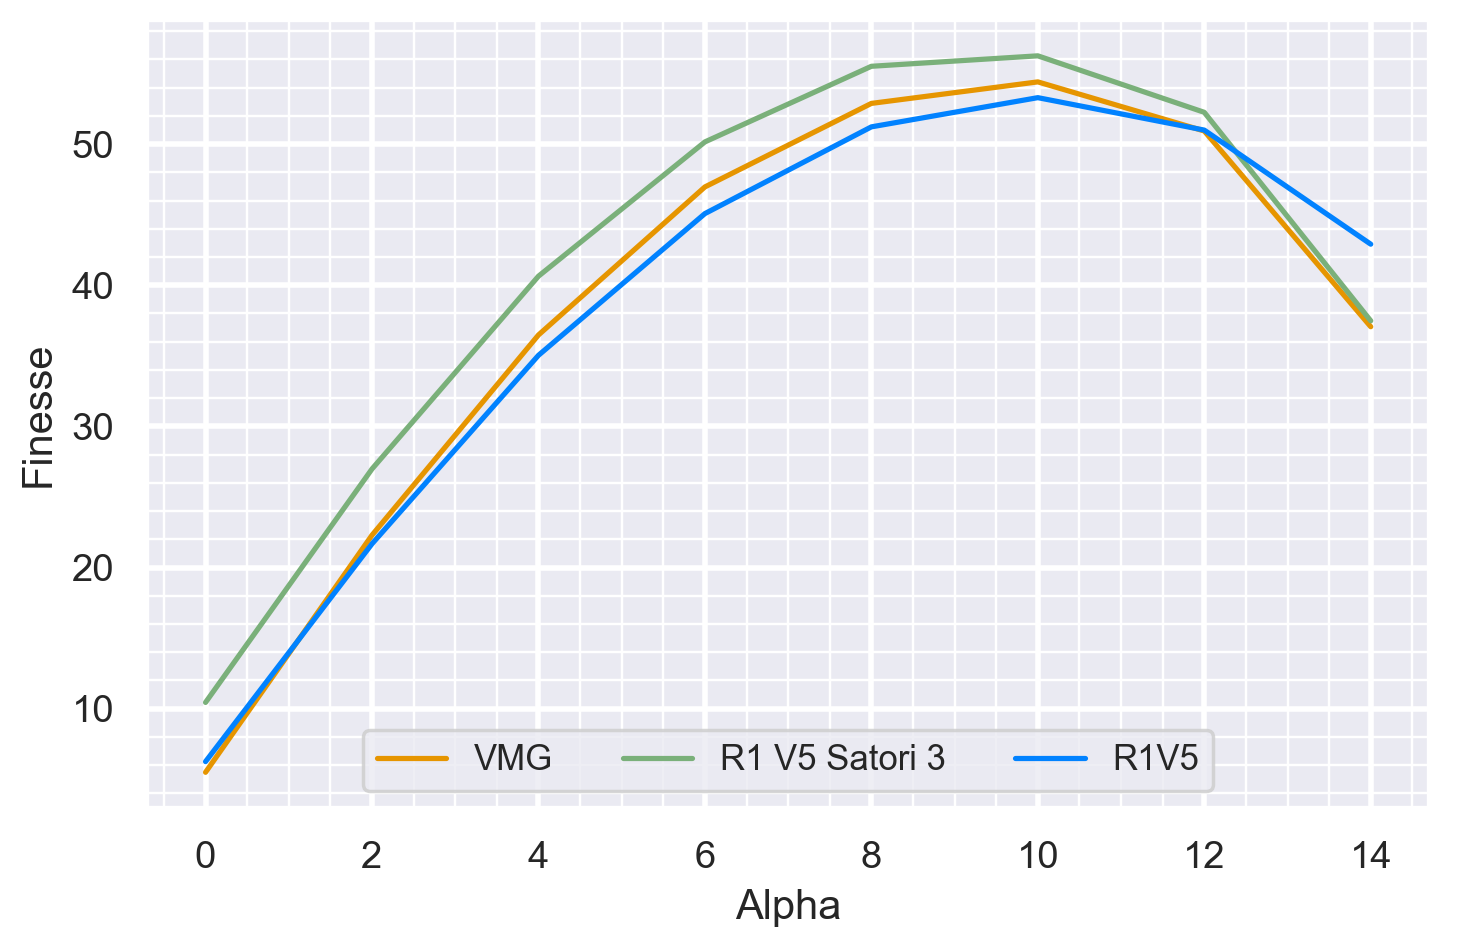
\includegraphics[width=1\textwidth]{figures/2D steady simulations/fluent/finesse VMG SAT3 R1V5 35kts FLUENT.png}
    \caption{35 knots}
    \label{fig:35 knots}
    \end{subfigure}
    \caption{R1 V5, R1 V5 Satori 3 \& VMG polars with FLUENT}
\label{fig:The R1 V5 meshing under FLUENT}
\end{figure}

These findings are rather promising, as we anticipate that the R1 V5 Satori3 will demonstrate enhanced performance in upwind conditions, particularly at low angles of attack, at 35 knots. Furthermore, in downwind scenarios, the R1 V5 Satori3 is projected to deliver favorable outcomes within the range of 5° to 8° angles of attack, but it is expected to experience a stall around 9-10°..  

\begin{figure}[H]
    \begin{subfigure}{0.5\textwidth}
    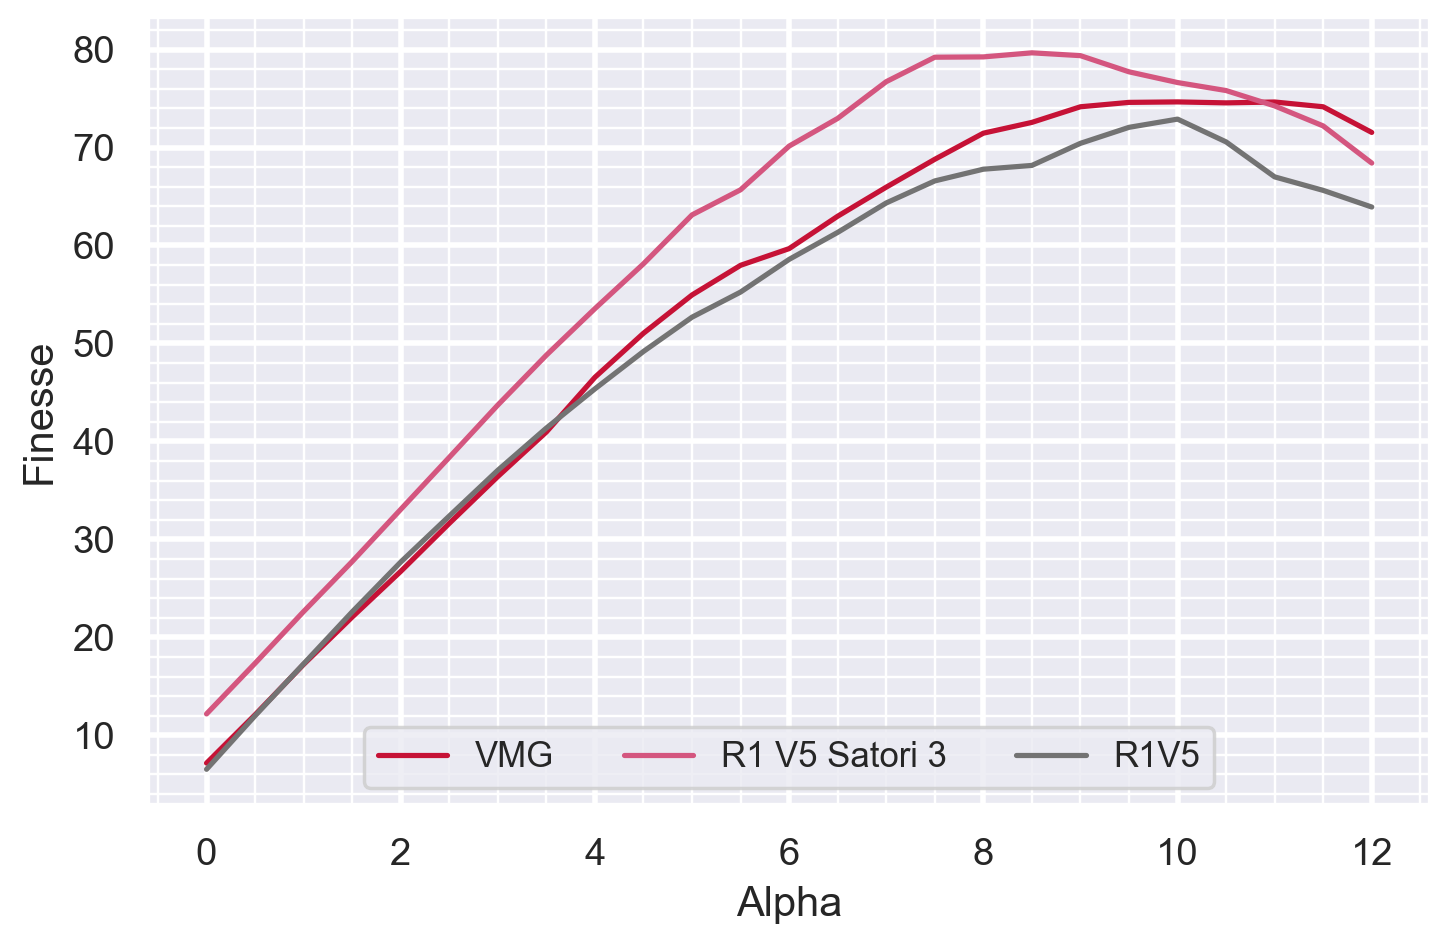
\includegraphics[width=1\textwidth]{figures/2D steady simulations/fluent/finesse VMG SAT3 R1V5 15kts XFLR5.png}
    \caption{15 knots}
    \label{fig:15 knots XFLR5}
    \end{subfigure}
    \begin{subfigure}{0.5\textwidth}
    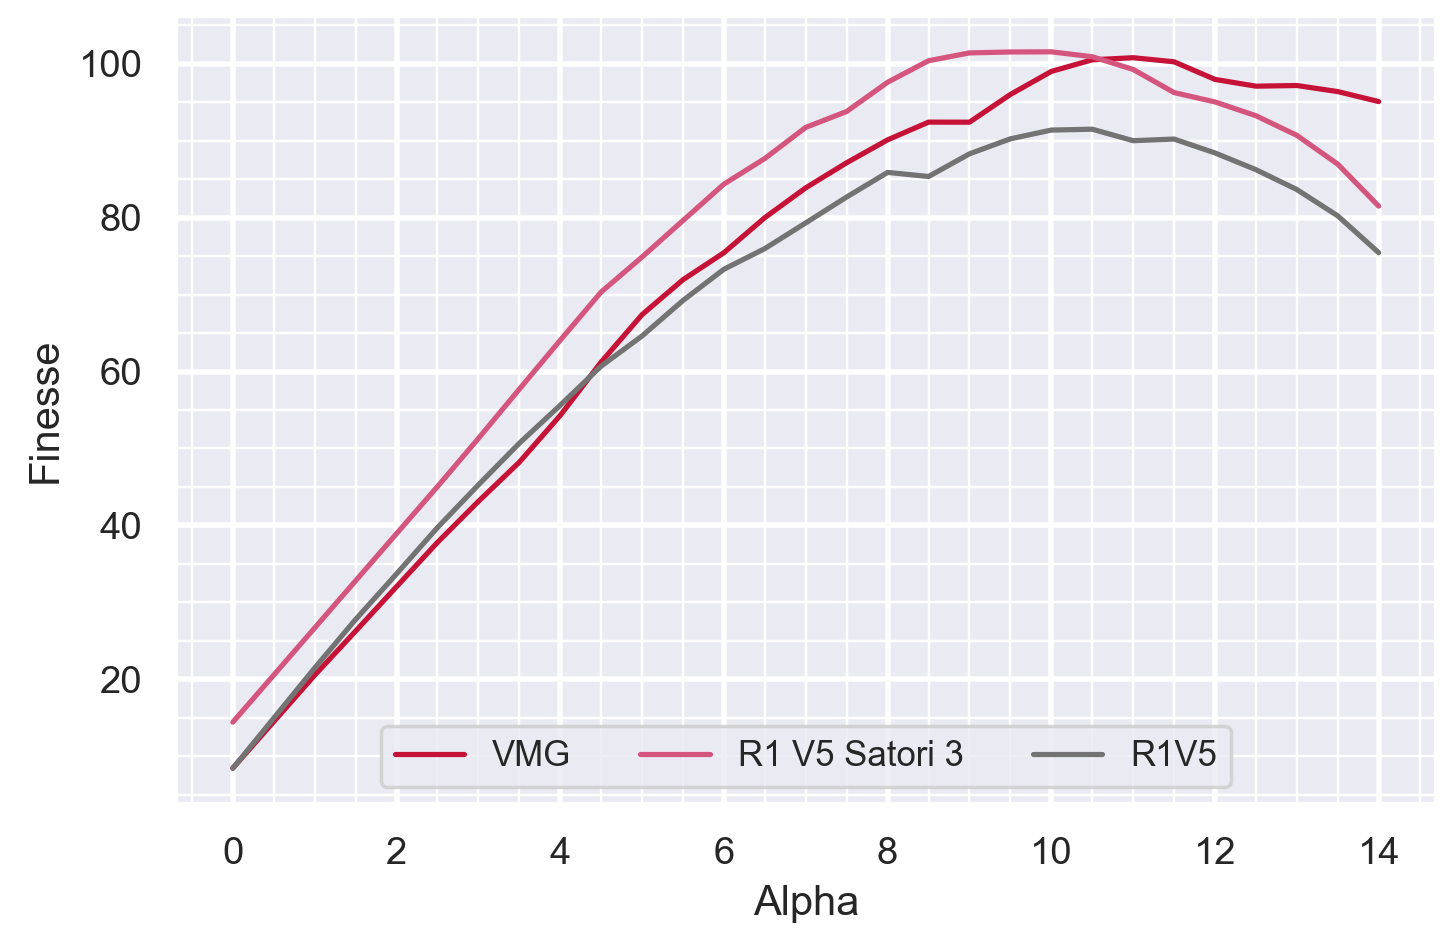
\includegraphics[width=1\textwidth]{figures/2D steady simulations/fluent/finesse VMG SAT3 R1V5 35kts XFLR5.png}
    \caption{35 knots}
    \label{fig:35 knots XFLR5}
    \end{subfigure}
    \caption{R1 V5, R1 V5 Satori 3 \& VMG polars with XFLR5}
\label{fig:The R1 V5 meshing under XFLR5}
\end{figure}

We also recognize the necessity of utilizing Fluent for simulations to achieve greater result accuracy, particularly when approaching the stall at high angles of attack. In fact, XFLR5 tends to provide higher estimates for the finesse values but is valuable for quickly obtaining initial insights into the relative behaviors of airfoils.

\textbf{The precision and cost-effectiveness of XFLR5 prompted, after extensive discussions with the paraglider design team, the initiation of a project to apply XFLR5's theories to simulate 3D effects and implement an optimization algorithm. This project is the central focus of Chapter \ref{Chapter2}.}

Consequently, we opted to initiate the development of a prototype for the R1 V5 Satori 3 and dispatch the kite to France for testing by the team riders to obtain their feedback on its performance.

\begin{figure}[H]
    \centering
    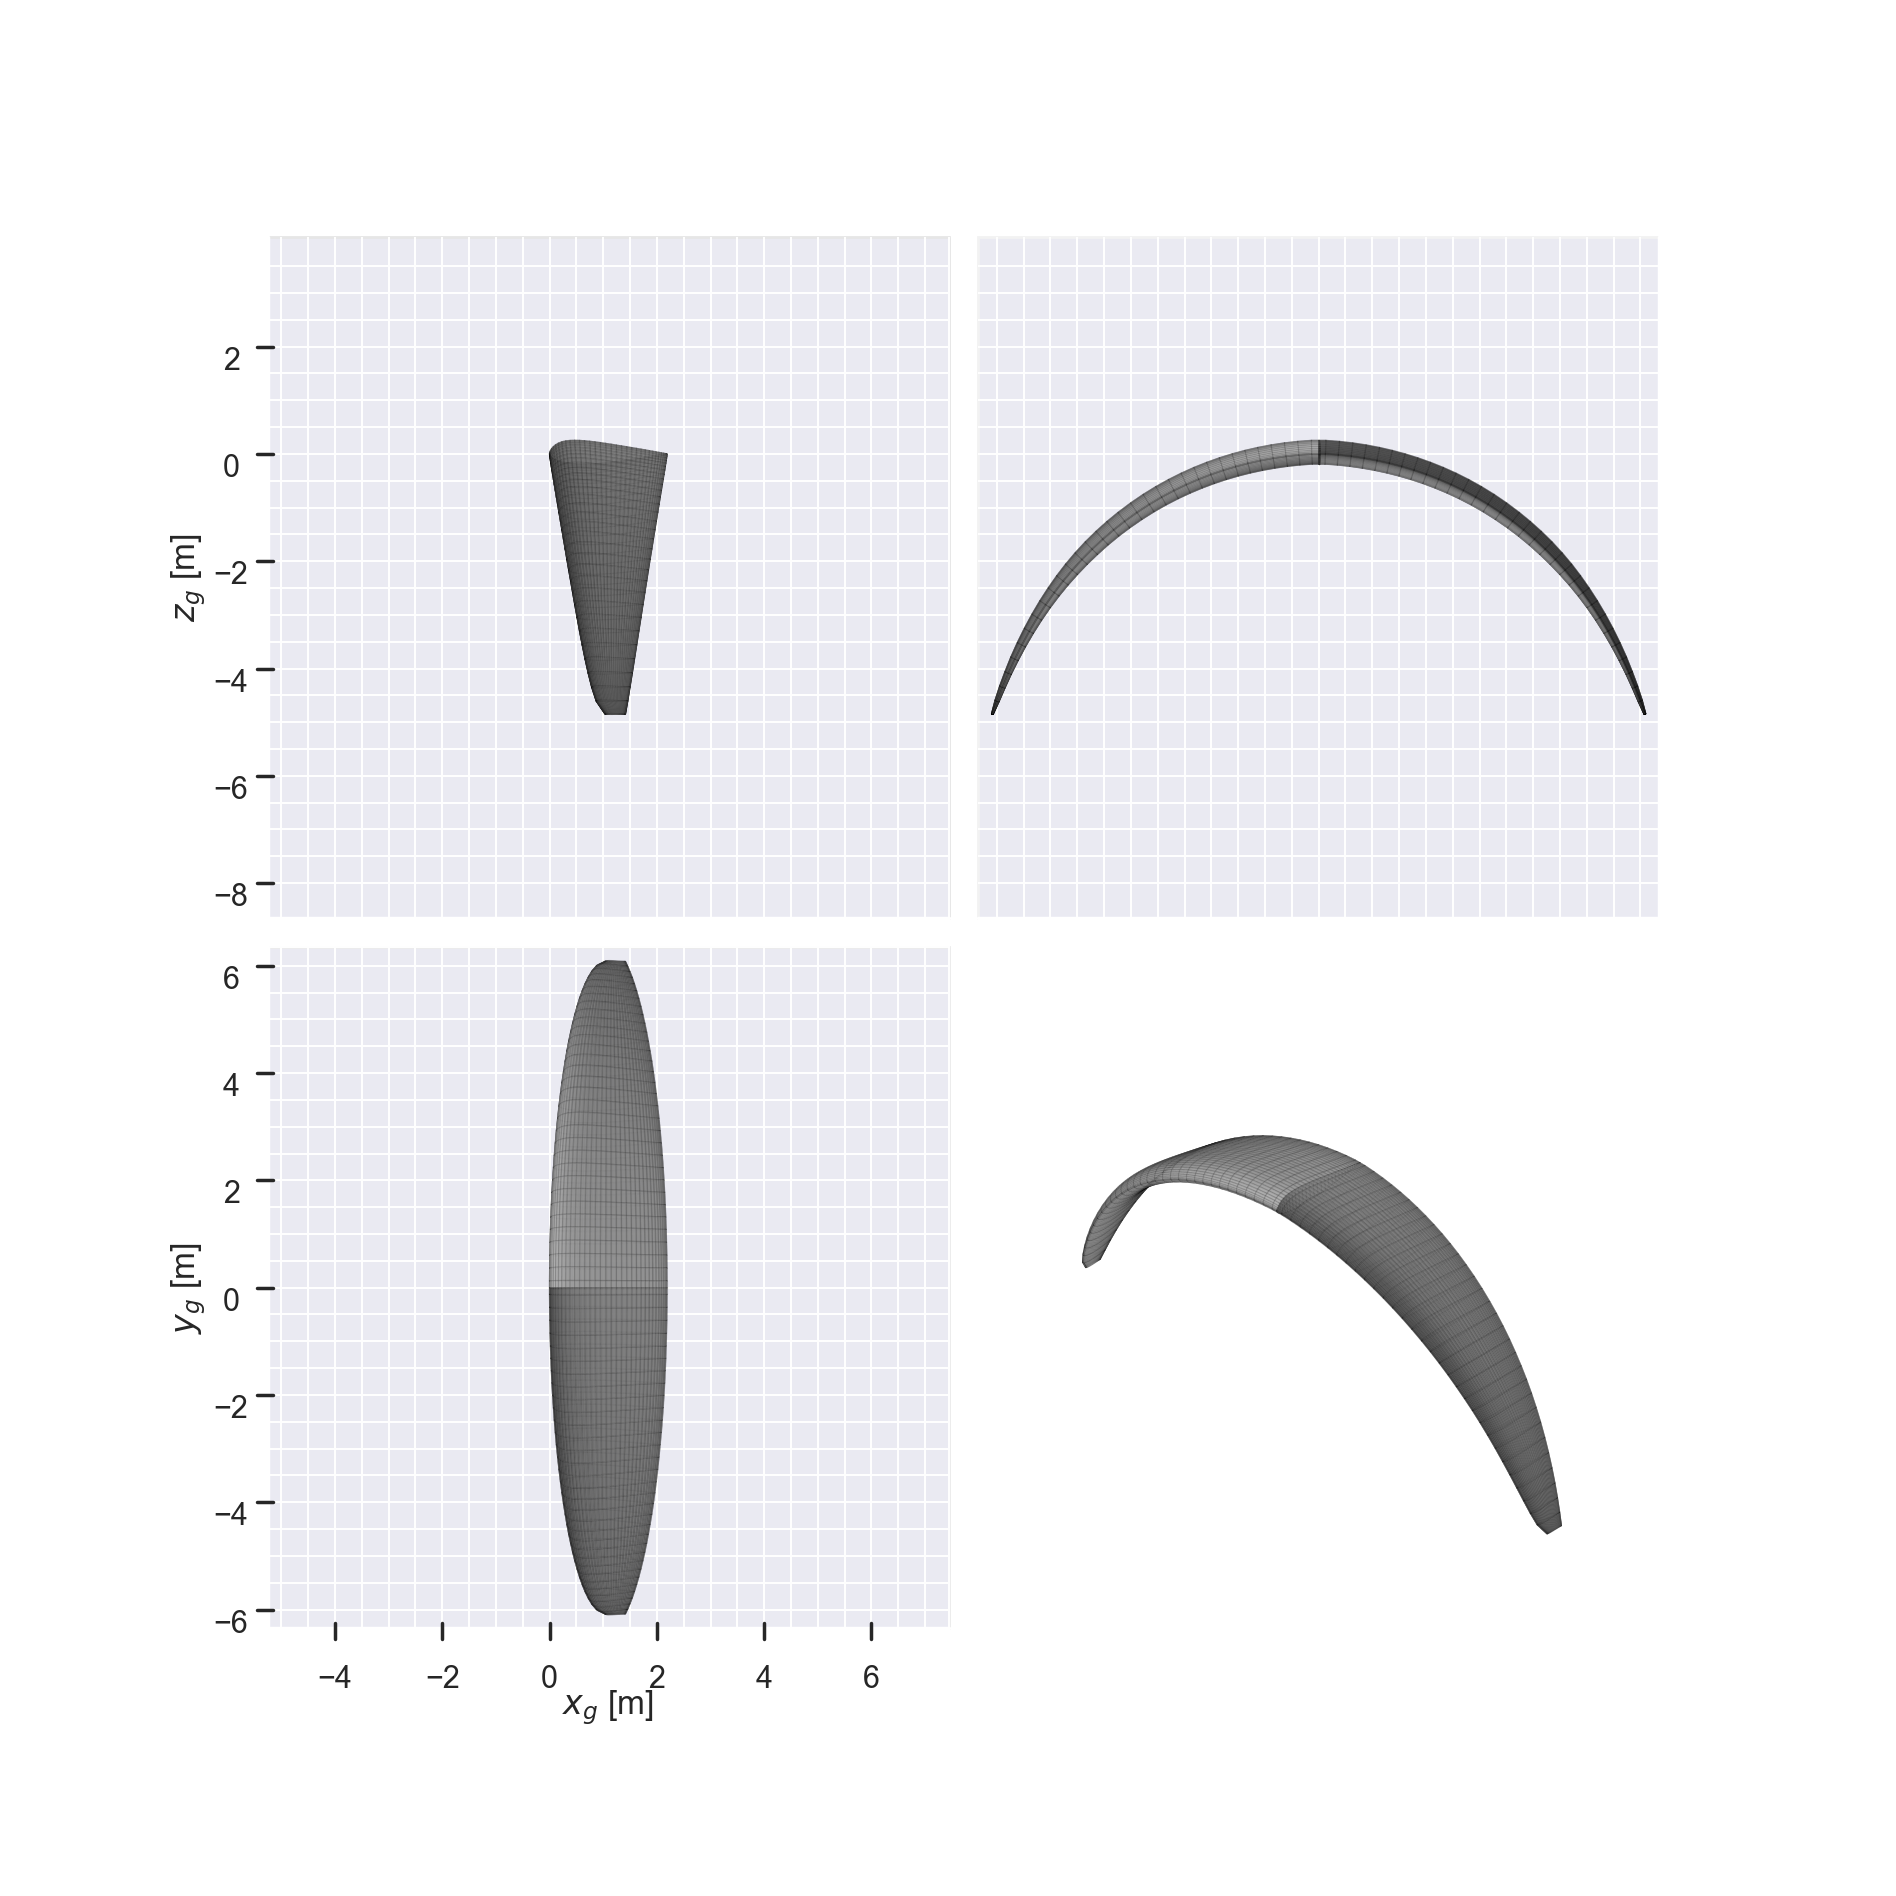
\includegraphics[width=1\linewidth]{figures/2D steady simulations/results/R1 V5 Satori 3 3D view.png}
    \caption{The R1 V5 Satori 3 3D view}
    \label{fig:The R1 V5 Satori 3 3D view}
\end{figure}

%%%%%%%%%%%%%%%%%%%%%%%%%%%%%%%%%%%% SUBSECTION 4

\subsection{The team rider feedbacks}
\label{sub:Ch1.6.4}

After several hours of adjustments and continuous use of the kite prototype until it reached its "final" shape (bearing in mind that the fabrics relax during the initial hours of testing), the team riders achieved higher Velocity Made Good (VMG) values upwind and maintained greater tether tension when going downwind. They enthusiastically declared that this kite was the most high-performing one they had ever tested and expressed optimism about the future of the kite we were developing.

Moreover, the accuracy in predicting kite performance and the alignment between theory and practice reassured the Ozone's design team about using science to shape their future kites. In fact, the kite surfing community has only recently embraced scientific knowledge in fluid mechanics, and these results served as Ozone's initial evidence of the value that numerical simulations can bring to the company.

It's important to note that many kites have benefited from my research on kite aerodynamics. This is because not all kites aim for the same performance characteristics. For instance, the smaller version of the R1 V5, which has an area of $11m^{2}$ compared to the $21m^{2}$ kite discussed in this report, is used in stronger winds where the emphasis is not on exploiting the finesse of the kite (as the wind is already strong, and other factors like the pilot's skill or the performance of the submerged foil in the water are limiting), but rather on its stability. As a result, the entirety of the work developed in this report has contributed to the development of this kite, which serves very different objectives, but for which the contribution of scientific research has proven to be beneficial. 

Once again, the feedback from the team riders during tests conducted on prototypes of these kites has proven to be in line with theory, and the kites developed in this manner have demonstrated higher performance than the existing ones.
